%% USEFUL LINKS:
%% -------------
%%
%% - UiO LaTeX guides:          https://www.mn.uio.no/ifi/tjenester/it/hjelp/latex/
%% - Mathematics:               https://en.wikibooks.org/wiki/LaTeX/Mathematics
%% - Physics:                   https://ctan.uib.no/macros/latex/contrib/physics/physics.pdf
%% - Basics of Tikz:            https://en.wikibooks.org/wiki/LaTeX/PGF/Tikz
%% - All the colors!            https://en.wikibooks.org/wiki/LaTeX/Colors
%% - How to make tables:        https://en.wikibooks.org/wiki/LaTeX/Tables
%% - Code listing styles:       https://en.wikibooks.org/wiki/LaTeX/Source_Code_Listings
%% - \includegraphics           https://en.wikibooks.org/wiki/LaTeX/Importing_Graphics
%% - Learn more about figures:  https://en.wikibooks.org/wiki/LaTeX/Floats,_Figures_and_Captions
%% - Automagic bibliography:    https://en.wikibooks.org/wiki/LaTeX/Bibliography_Management  (this one is kinda difficult the first time)
%%
%%                              (This document is of class "revtex4-1", the REVTeX Guide explains how the class works)
%%   REVTeX Guide:              http://www.physics.csbsju.edu/370/papers/Journal_Style_Manuals/auguide4-1.pdf
%%
%% COMPILING THE .pdf FILE IN THE LINUX IN THE TERMINAL
%% ----------------------------------------------------
%%
%% [terminal]$ pdflatex report_example.tex
%%
%% Run the command twice, always.
%%
%% When using references, footnotes, etc. you should run the following chain of commands:
%%
%% [terminal]$ pdflatex report_example.tex
%% [terminal]$ bibtex report_example
%% [terminal]$ pdflatex report_example.tex
%% [terminal]$ pdflatex report_example.tex
%%
%% This series of commands can of course be gathered into a single-line command:
%% [terminal]$ pdflatex report_example.tex && bibtex report_example.aux && pdflatex report_example.tex && pdflatex report_example.tex
%%
%% ----------------------------------------------------


\documentclass[english,notitlepage,reprint,nofootinbib]{revtex4-1}  % defines the basic parameters of the document
% For preview: skriv i terminal: latexmk -pdf -pvc filnavn
% If you want a single-column, remove "reprint"

% Allows special characters (including æøå)
\usepackage[utf8]{inputenc}
% \usepackage[english]{babel}

%% Note that you may need to download some of these packages manually, it depends on your setup.
%% I recommend downloading TeXMaker, because it includes a large library of the most common packages.

\usepackage{physics,amssymb}  % mathematical symbols (physics imports amsmath)
\include{amsmath}
\usepackage{graphicx}         % include graphics such as plots
\usepackage{xcolor}           % set colors
\usepackage{hyperref}         % automagic cross-referencing
\usepackage{listings} % display code
\usepackage{subfigure}        % imports a lot of cool and useful figure commands
% \usepackage{float}
%\usepackage[section]{placeins}
\usepackage{algorithm}
\usepackage[noend]{algpseudocode}
\usepackage{subfigure}
\usepackage{tikz}
\usepackage{mathtools}
\usepackage{nccmath}
\usepackage{comment}
\usepackage{natbib}
\usetikzlibrary{quantikz}
\parskip=5pt plus 1pt
% defines the color of hyperref objects
% Blending two colors:  blue!80!black  =  80% blue and 20% black
\hypersetup{ % this is just my personal choice, feel free to change things
    colorlinks,
    linkcolor={red!50!black},
    citecolor={blue!50!black},
    urlcolor={blue!80!black}}

% ===========================================


\begin{document}

\title{\LARGE{Project 3 on Machine Learning}\\
  \large{Logistic Regression, Deep Neural Network \\ and Support Vector Machine by comparison}}
\author{Adele Zaini}
\thanks{GitHub profile: \href{https://github.com/adelezaini/}{ https://github.com/adelezaini/}}
\date{\today}
\noaffiliation                            % ignore this, but keep it.

\maketitle
\section*{Abstract}

A comparison between the three Machine Learning techniques of Logistic Regression, Neural Network and Support Vector Machine is presented. Their performance is evaluated in a classification case, using the Climate Models Simulation Crashes dataset from the UCI repository, that explores the failures in running climate models ensembles when perturbating different input parameters. The combination of Machine Learning techniques in climate sciences is rising in importance in the recent decades, due to the stochastic component of the atmosphere that is demanding in modelling using the standard techniques. In this work, a side case of using machine learning techniques to find an apparently non-deterministic pattern in evaluating climate models limitations is here presented. Evaluating the performance of the three techniques, the Neural Network is the one that predicts better when the climate model could fail with an accuracy score of $96.1\%$ and $10$ failures correctly predicted out of the $14$ expected. The accuracy scores of the Logistic Regression and the Support Vector Machine are respectively of 92.8\%, and 92.2\%, which seem high, but looking at the failures hit only, they fail in this prediction. The Neural Network performance is also improved when optimizing the hidden activation functions and the optimizers, reaching almost the $98\%$ of accuracy score with the combination of \textit{elu} and \textit{sgd} respectively.


% ===========================================
\section{Introduction}
Machine Learning techniques are expanding in all the fields of research in the last decades and have led to important improvements. One of this field belongs to the Climate Sciences, where studying the stochastic behaviour of the atmosphere is not possible with only the classical methods. These techniques are also useful to learn about further insights on side topics, such as uncertainty quantification (UQ) simulations, and to improve the Earth System Models themselves.

In this report we will compare three different Machine Learning techniques applied to a classification dataset realized by climate simulations (Section \ref{sec:data}). After implementing Logistic Regression, Neural Network and Support Vector Machine, their performance will be quantified and compared. The second part of the analysis focuses instead on optimizing the Neural Network, finding the best combination between the activation function of the hidden layers and the optimizer.

The report is organized as follows. After this introduction, an insight of the dataset is presented (\textit{part a}\footnote{The project text divides the work in five parts, in this work these parts are sections of the report, following the given order.}), followed by the theory around the machine learning techniques (\textit{part b}) and the algorithms implemented (\textit{part c}). The following section will present the results of the work (\textit{part d}), while commenting and discussing them. The final section is to summarize the analysis into the conclusions and to have an overview on future perspectives (\textit{part e}).


    
% ===========================================
\section{Data}\label{sec:data} 

Since my interest in Climate Modelling, the dataset used in this work is taken from the University of California at Irvine (UCI) repository   and deals with the analysis of crashes in Climate Models Ensembles when perturbating different input parameters. The dataset is called \textit{Climate Model Simulation Crashes} and on the UCI website all the information about this dataset and its structure can be found (Ref. \cite{UCI}).


\textbf{Motivation} 
This dataset was created to respond to an emergent finding when analysing the effects of ocean model parameter uncertainties on climate simulations: a series of simulation crashes within the Parallel Ocean Program (POP2) component of the Community Climate System Model version 4 (CCSM4). About 8.5\% of the CCSM4 simulations failed for numerical reasons at combinations of POP2 parameter values. D.D. Lucas et al. \cite{failure} created the present dataset composed by the parameters values and the outcomes (success, failure) for each run, in order to find a pattern in the multidimensional space of parameters using the Support Vector Machine technique and to better understand the reasons underlying the problem.

\textbf{Climate Models and UQ ensembles} Modern global three-dimensional climate models are extraordinarily complex pieces of science. They contain over a million lines of code and use hundreds to thousands of functions and subroutines to solve equations of state and conservation laws for the flows of matter, energy, and momentum within and between the atmosphere, oceans, land, and other reservoirs of the Earth system. They also use numerous algorithms of biological, chemical, geologic, and anthropogenic processes to simulate the cycles of carbon, nitrogen, sulfur, aerosols, ozone, greenhouse gases and other climate components. Given this enormous complexity, climate models are vulnerable to many types of computational issues. As code verification can be used to find software bugs, emerging tools being developed in the field of uncertainty quantification (UQ) can help pinpoint scientific discrepancies in simulation models, the knowledge of which can be used to guide and improve model development. Primary UQ targets for climate models are schemes containing parameters with adjustable values. This type of simulations are called \textit{Perturbed Parameter Ensemble} (PPE). Small perturbations to the values of the parameters can amplify and lead to large changes in simulation outputs. In some cases, the simulations may fail altogether. The present dataset reports a series of simulation crashes encountered while running perturbed parameter UQ ensembles of the Community Climate System Model Version 4 (CCSM4) (Ref.\cite{failure}).

\textbf{Dataset structure}
In spite of the complexity underlying these climate model simulations, the authors of the dataset treat the crash problem as a black box where just the values of the input parameters and a binary outcome flag indicating whether the simulations failed or were completed are known. In order to generate this dataset, three separate Latin hypercube ensembles were conducted, each containing 180 ensemble members, given 18 different parameters as input. 46 out of the total 540 simulations failed for numerical reasons at combinations of parameter values.
The description of the columns of the dataset is the following:

\begin{itemize}
    \item[–] \textit{Col 1 - "Study"}: Latin hypercube study ID (study 1 to 3).
    \item[–] \textit{Col 2 - "Run"}: simulation ID (run 1 to 180)
    \item[–] \textit{Cols 3-20 - variable names}: values of 18 climate model parameters scaled in the interval [0, 1]
    \item[–] \textit{Col 21 - "outcome"}: simulation outcome (0 = failure, 1 = success)
\end{itemize}

For a basic explanation of the Latin hypercube you can check \cite{latinwiki} and for further mathematical insights look at Z. Liu et at., 2015 \cite{latin}.

The \textit{variable names} are listed in the Table \ref{fig:big_table}, for further details look at the complete table in the Appendix \ref{sec:appendix}.

\begin{figure}[h]
    \centering 
    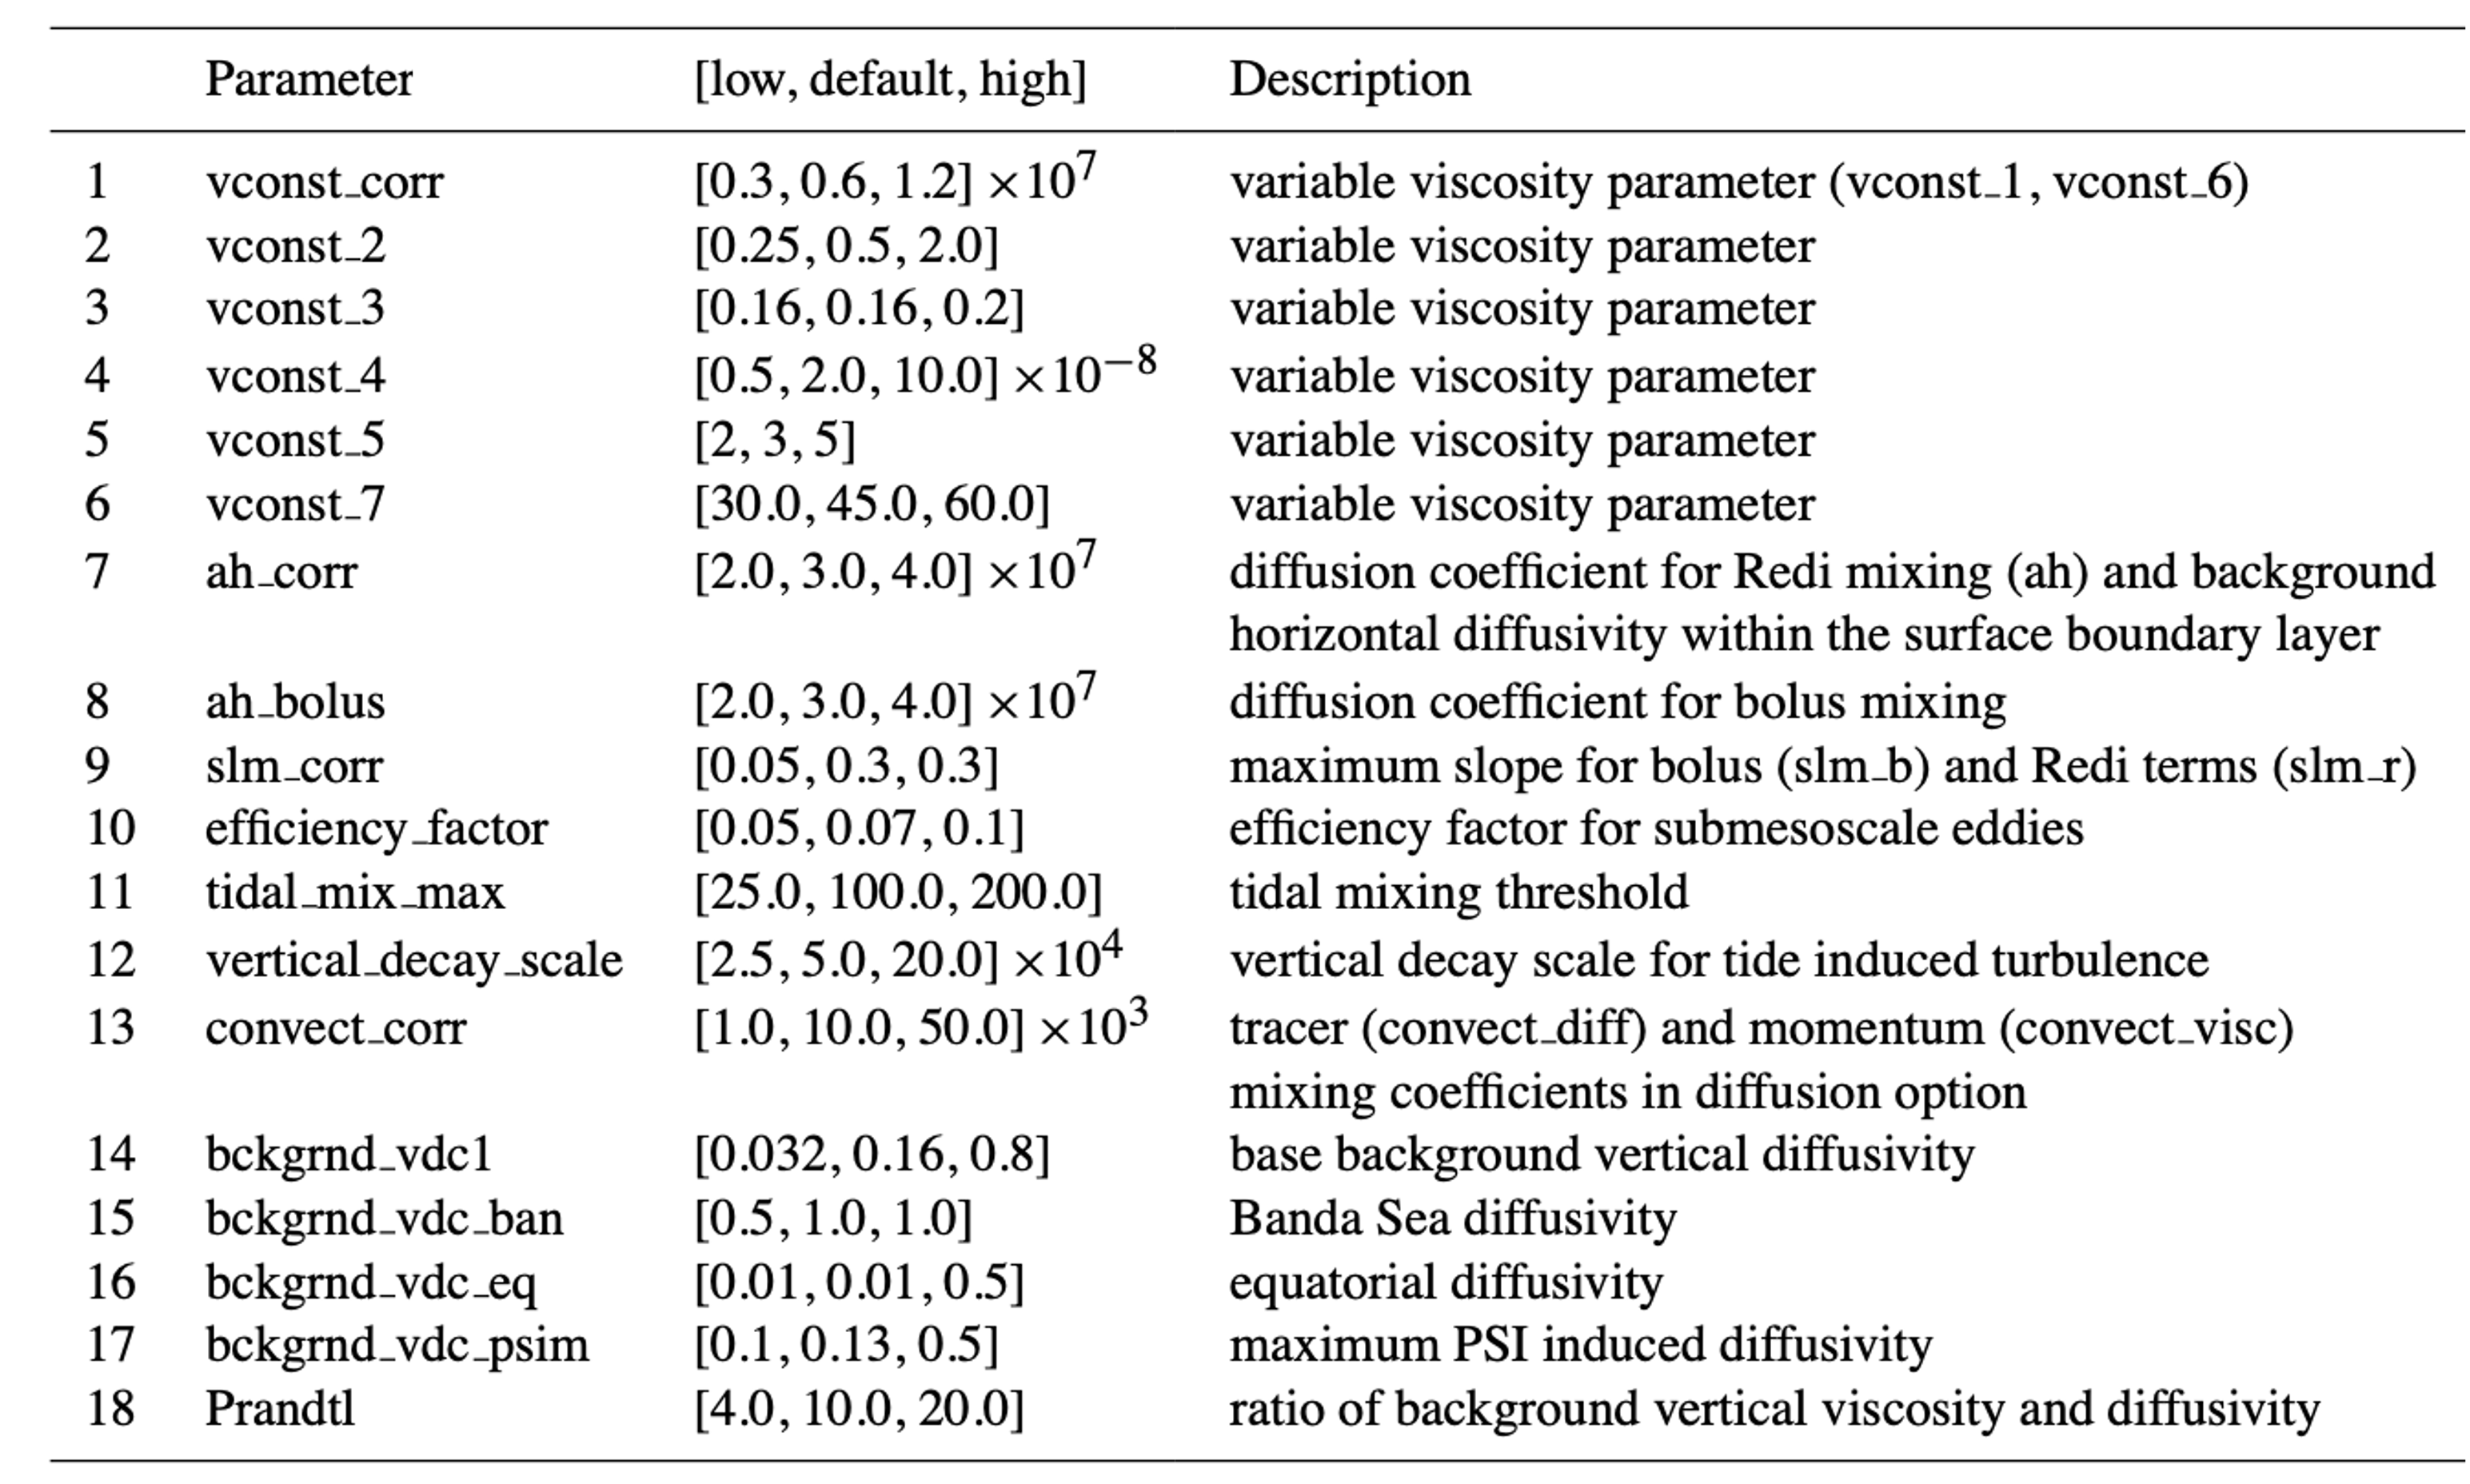
\includegraphics[scale=0.35]{img/big_table.png}
    \caption{Description of the 18 features. Note: individual corr parameters (numbers 1, 7, 9, and 13) are used to represent the correlated pair of parameters given in the description. For example, values drawn for vconst corr are assigned to vconst 1 and vconst 6. b Linear and logarithmic scales are used for parameter ranges that have ratios of high/low < 5 and high/low ≥ 5, respectively. For the complete table look in the Appendix (Ref. \cite{failure})}
    \label{fig:big_table}
\end{figure}

Note that the dataset parameters are already scaled in the interval [0,1], so they will not be rescaled in the process. In the splitting for training and test data, the studies 1 and 2 are taken into the training dataset, while study 3 is considered to test the model performance.

\textbf{Dataset analysis}

\begin{figure}[h]
    \centering 
    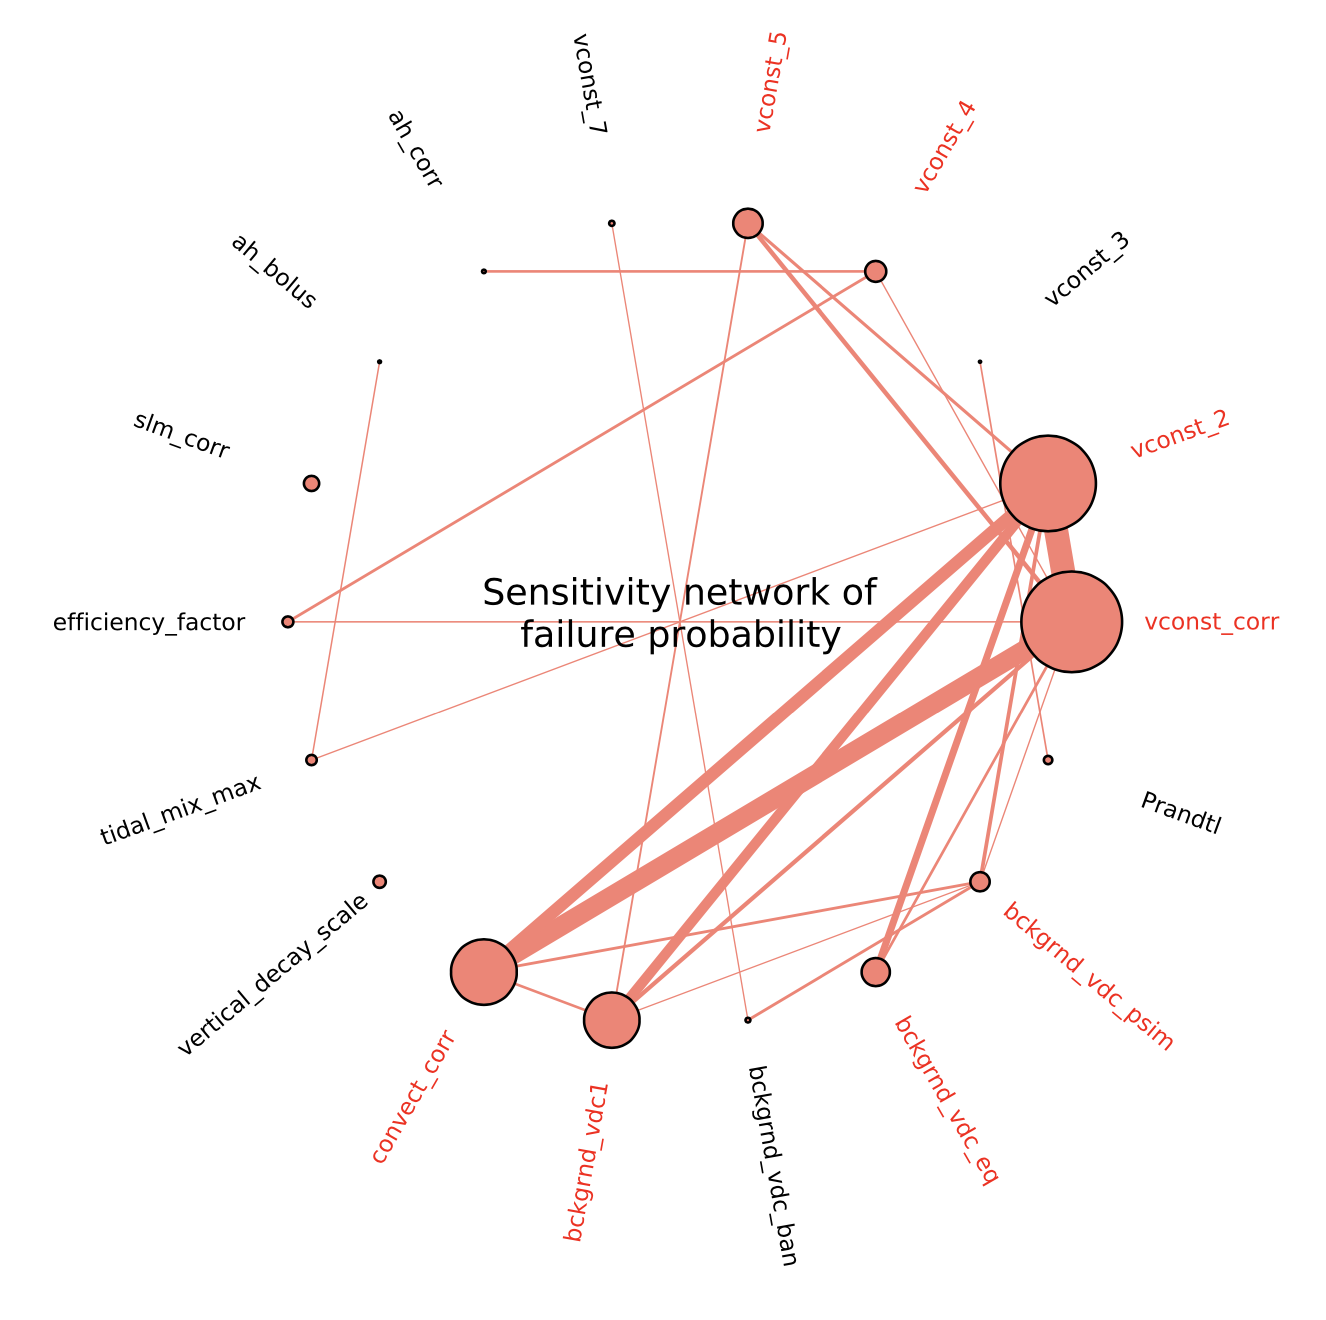
\includegraphics[scale=0.28]{dataset/sensitivity.png}
    \caption{Sensitivity analysis performed on the 18 perturbed parameters, showing which are the most important relationships with the outcome (Ref. \cite{failure}).}
    \label{data:sens}
\end{figure}


\begin{figure}[h]
    \centering 
    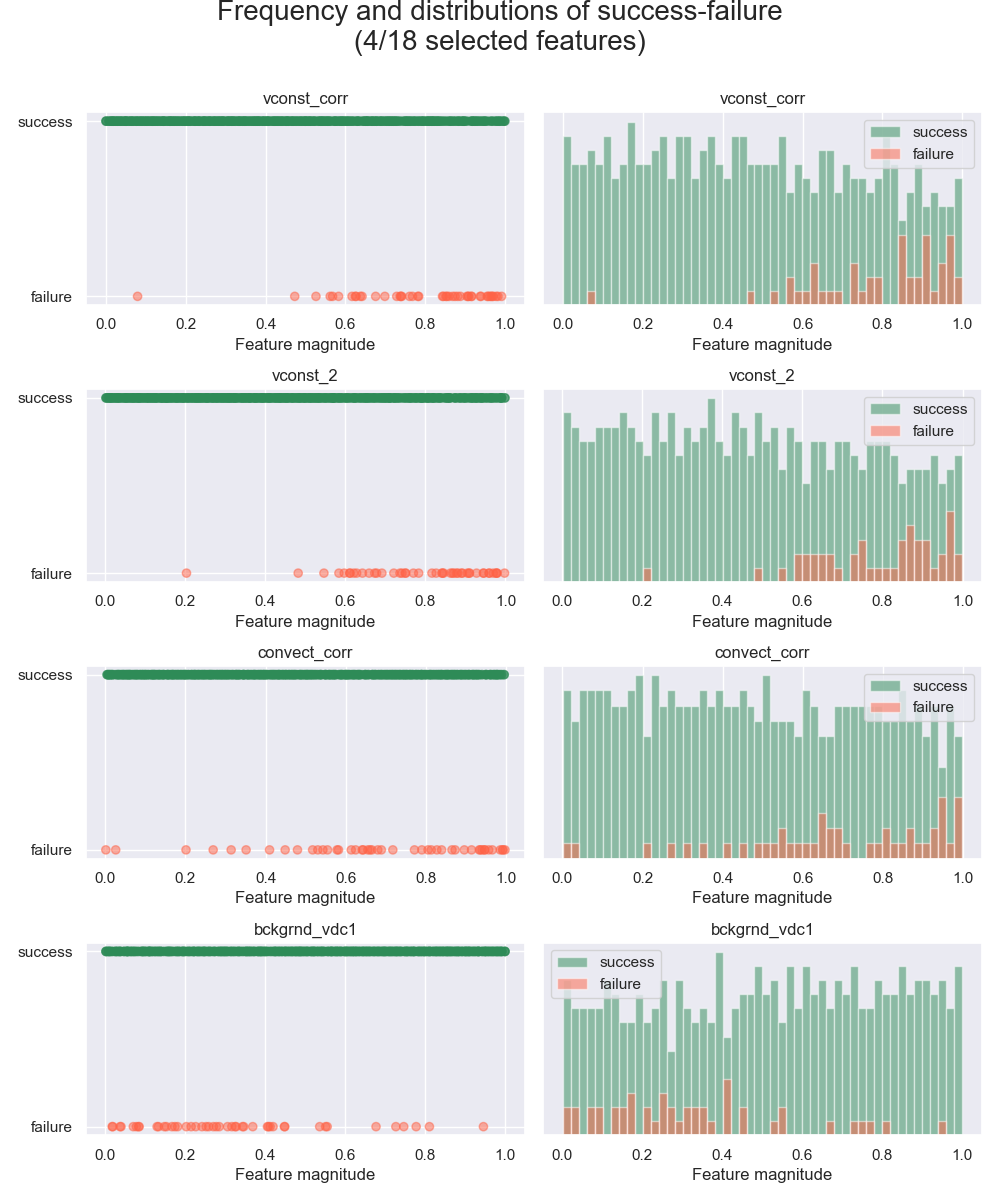
\includegraphics[scale=0.3]{dataset/distributions_sel.png}
    \caption{Frequency and distribution of the outcomes for the 4 most sensible parameters (Figure \ref{data:sens}).}
    \label{data:1d}
\end{figure}
\begin{figure}[h]
    \centering 
    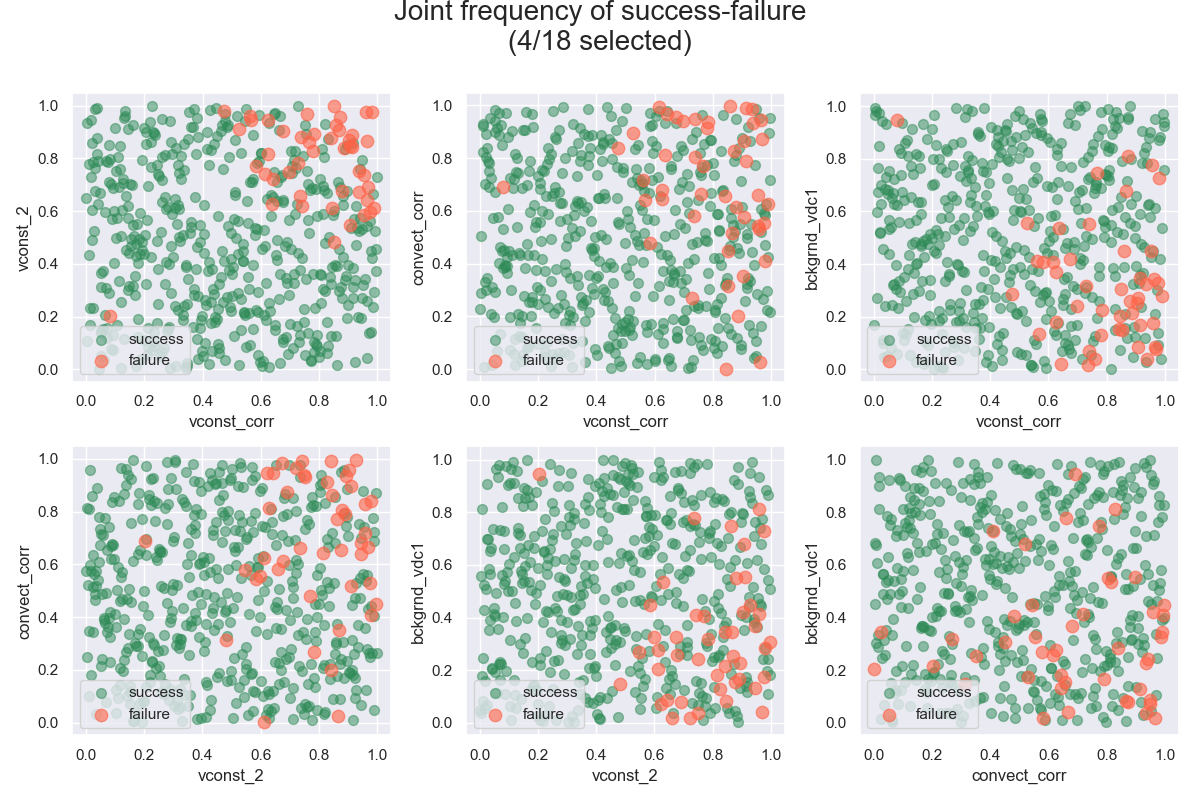
\includegraphics[scale=0.28]{dataset/distributions_2D_sel.png}
    \caption{2D frequency of the outcomes for combinations of the 4 most sensible parameters (Figure \ref{data:sens}).}
    \label{data:2d}
\end{figure}


Figure \ref{data:corr} shows a very little correlation among the data and . Note that very narrow colorscale is set in order to appreciate the little differences.

Analysing the frequency and the distribution of the success-failure per parameter, most of the parameters do not show any particular behaviour in relation to the simulation crashes. In Figures \ref{data:1d} and \ref{data:2d} just the four most sensible parameters are selected, based on the study \cite{failure} shown in Figure \ref{data:sens}. Figure \ref{data:1d} represents the frequency and distribution of success-failure for each of \textit{'vconst\_corr', 'vconst\_2', 'convect\_corr', 'bckgrnd\_vdc1'} (refer to Table \ref{fig:big_table} for variable complete names), while Figure \ref{data:2d} shows the joint frequency taken couples out of these four parameters to better show the relationship to the success of the simulations. We can then notice that the probability that model crashes increase when increasing values of \textit{'vconst\_corr', 'vconst\_2', 'convect\_corr'} and decreasing values of \textit{'bckgrnd\_vdc1'}. For further physical interpretation of these behaviours, look at Lucas D. D. et al. \cite{failure}. Here it is not reported since it is a discussion that goes further than the objectives of this work. The complete table with all the paramaters analysis can be found in the Appendix (Figure \ref{data:tot}). It is not shown here to keep the discussion brief and for pointing out the important relationships. 

Since there are 18 features in this dataset, our objective can be finding correlations among the data in order to condense the information in fewer parameters and decrease the dimensionality of the problem. To do so, the selected technique is the Principal Component Analysis (PCA), that will be discussed in details in the next section \ref{sec:theory}.

\begin{figure}[h]
    \centering 
    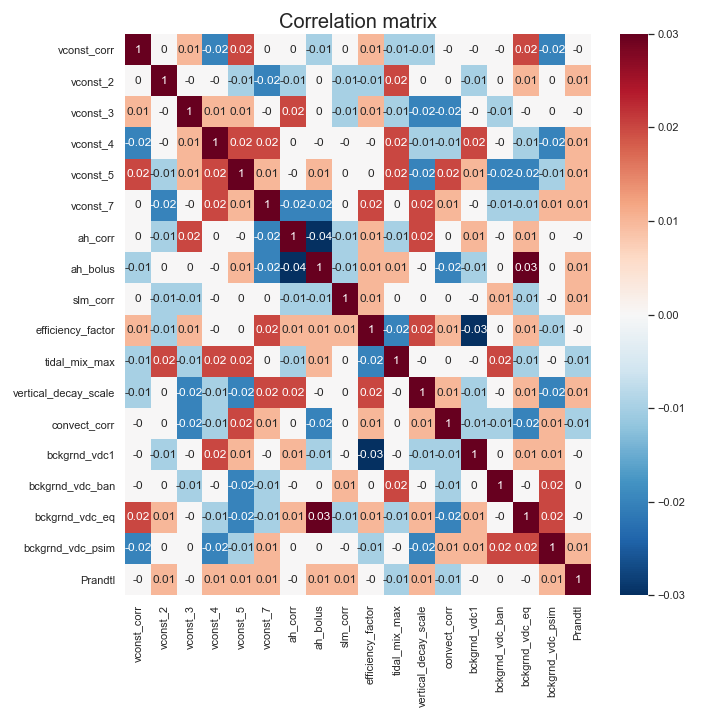
\includegraphics[scale=0.3]{dataset/correlationmatrix.png}
    \caption{Correlation matrix for the 18 perturbed parameters. Note that the color scale is set in the narrow range $[-0.03,0.03]$.}
    \label{data:corr}
\end{figure}

The first step is having an overview on the correlations among data: the more correlations there are, the more the information can be concentrated in fewer variables. The Figure \ref{data:corr} shows though that the data are very little correlated and any significant correlation can be found (the highest is $0.04$). Note that the color scale is very narrow to appreciate the small differences. In this specific case, applying the PCA can lead to little improvements in terms of dimensionality reduction. This is indeed confirmed by performing the PCA setting different cumulative variances, instead of choosing \textit{a priori} the number of Principal Components (see Section \ref{sec:theory}). With a cumulative variance of 95\%, all the 18 features are kept and even lowering the variance the result doesn't enhance the possibility of reducing the dimensionality. This then lead to the conclusion that in this specific case it is not possible to reduce the number of variables, otherwise too much information would be lost. 


\section{Theory} \label{sec:theory}
In this section, some background theory is presented to better understand the Machine Learning techniques implemented in this work, together with insights on the algorithms of each technique. Since in this work the code used methods from Scikit-Learn \cite{sk} and Tensorflow \cite{tf}, the algorithms are just sketched theoretically (reason why they are in this section), but we suggest to refer to the documentation of these packages for specific implementations of these algorithms.

\subsection{Principal Component Analysis} \label{sec:pc}

Principal component analysis (PCA) is a statistical technique for dimension reduction. In practice, it is used when there are variables related to each other within a dataset and the aim is to reduce the number of data by losing the least amount of information possible.
The PCA has the objective of maximizing the variance, calculating the weight to be given to each input variable in order to condense them in one or more new variables (called Principal Components) that will be the linear combination of the original variables.
The accurancy score will decrease because we loose little information, but reducing the dimensionality can lead to many advantages, such as computational efficiency and specific model performance (Ref. \cite{pc1}, \cite{pc}).

\textbf{Principal Components}
The Principal components are new variables that are constructed as linear combinations of the initial variables. These combinations are done in such a way that the new variables are uncorrelated and most of the information within the initial variables is squeezed or compressed into the first components. So, the idea is $p$-dimensional data gives you $p$ principal components, but PCA tries to put maximum possible information in the first component, then maximum remaining information in the second and so on, until having something, as shown in Figure \ref{fig:PC}.

\begin{figure}[h]
    \centering 
    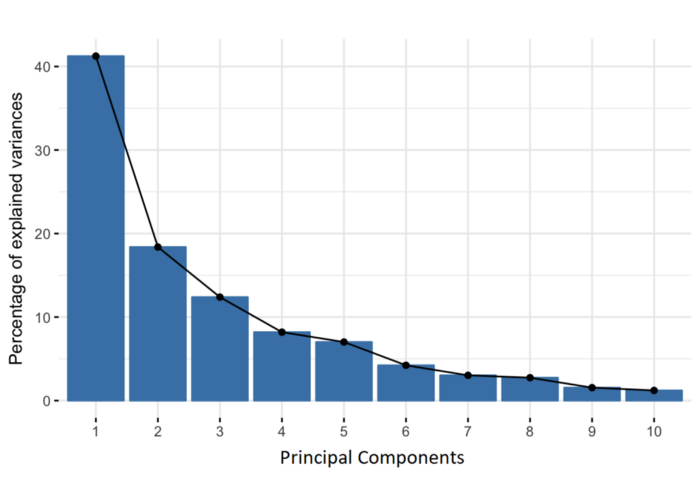
\includegraphics[scale=0.3]{img/principal_components.png}
    \caption{Percentage of Variance (Information) for each by principal components. The first two are here selected and account for about $60\%$ of the total variance (Ref. \ref{}).}
    \label{fig:PC}
\end{figure}

Organizing information in principal components this way, will allow to reduce dimensionality without losing much information, and this by discarding the components with low information and considering the remaining components as your new variables (Ref. \cite{pc}).

An important thing to realize here is that the principal components don’t have any real meaning since they are constructed as linear combinations of the initial variables.

Geometrically speaking, principal components represent the directions of the data that explain a maximal amount of variance, that is to say, the lines (or hyperplane in high dimension space) that capture most information of the data (Figure \ref{fig:PC2}, Ref. \cite{mortens}). 


\begin{figure}[h]
    \centering 
    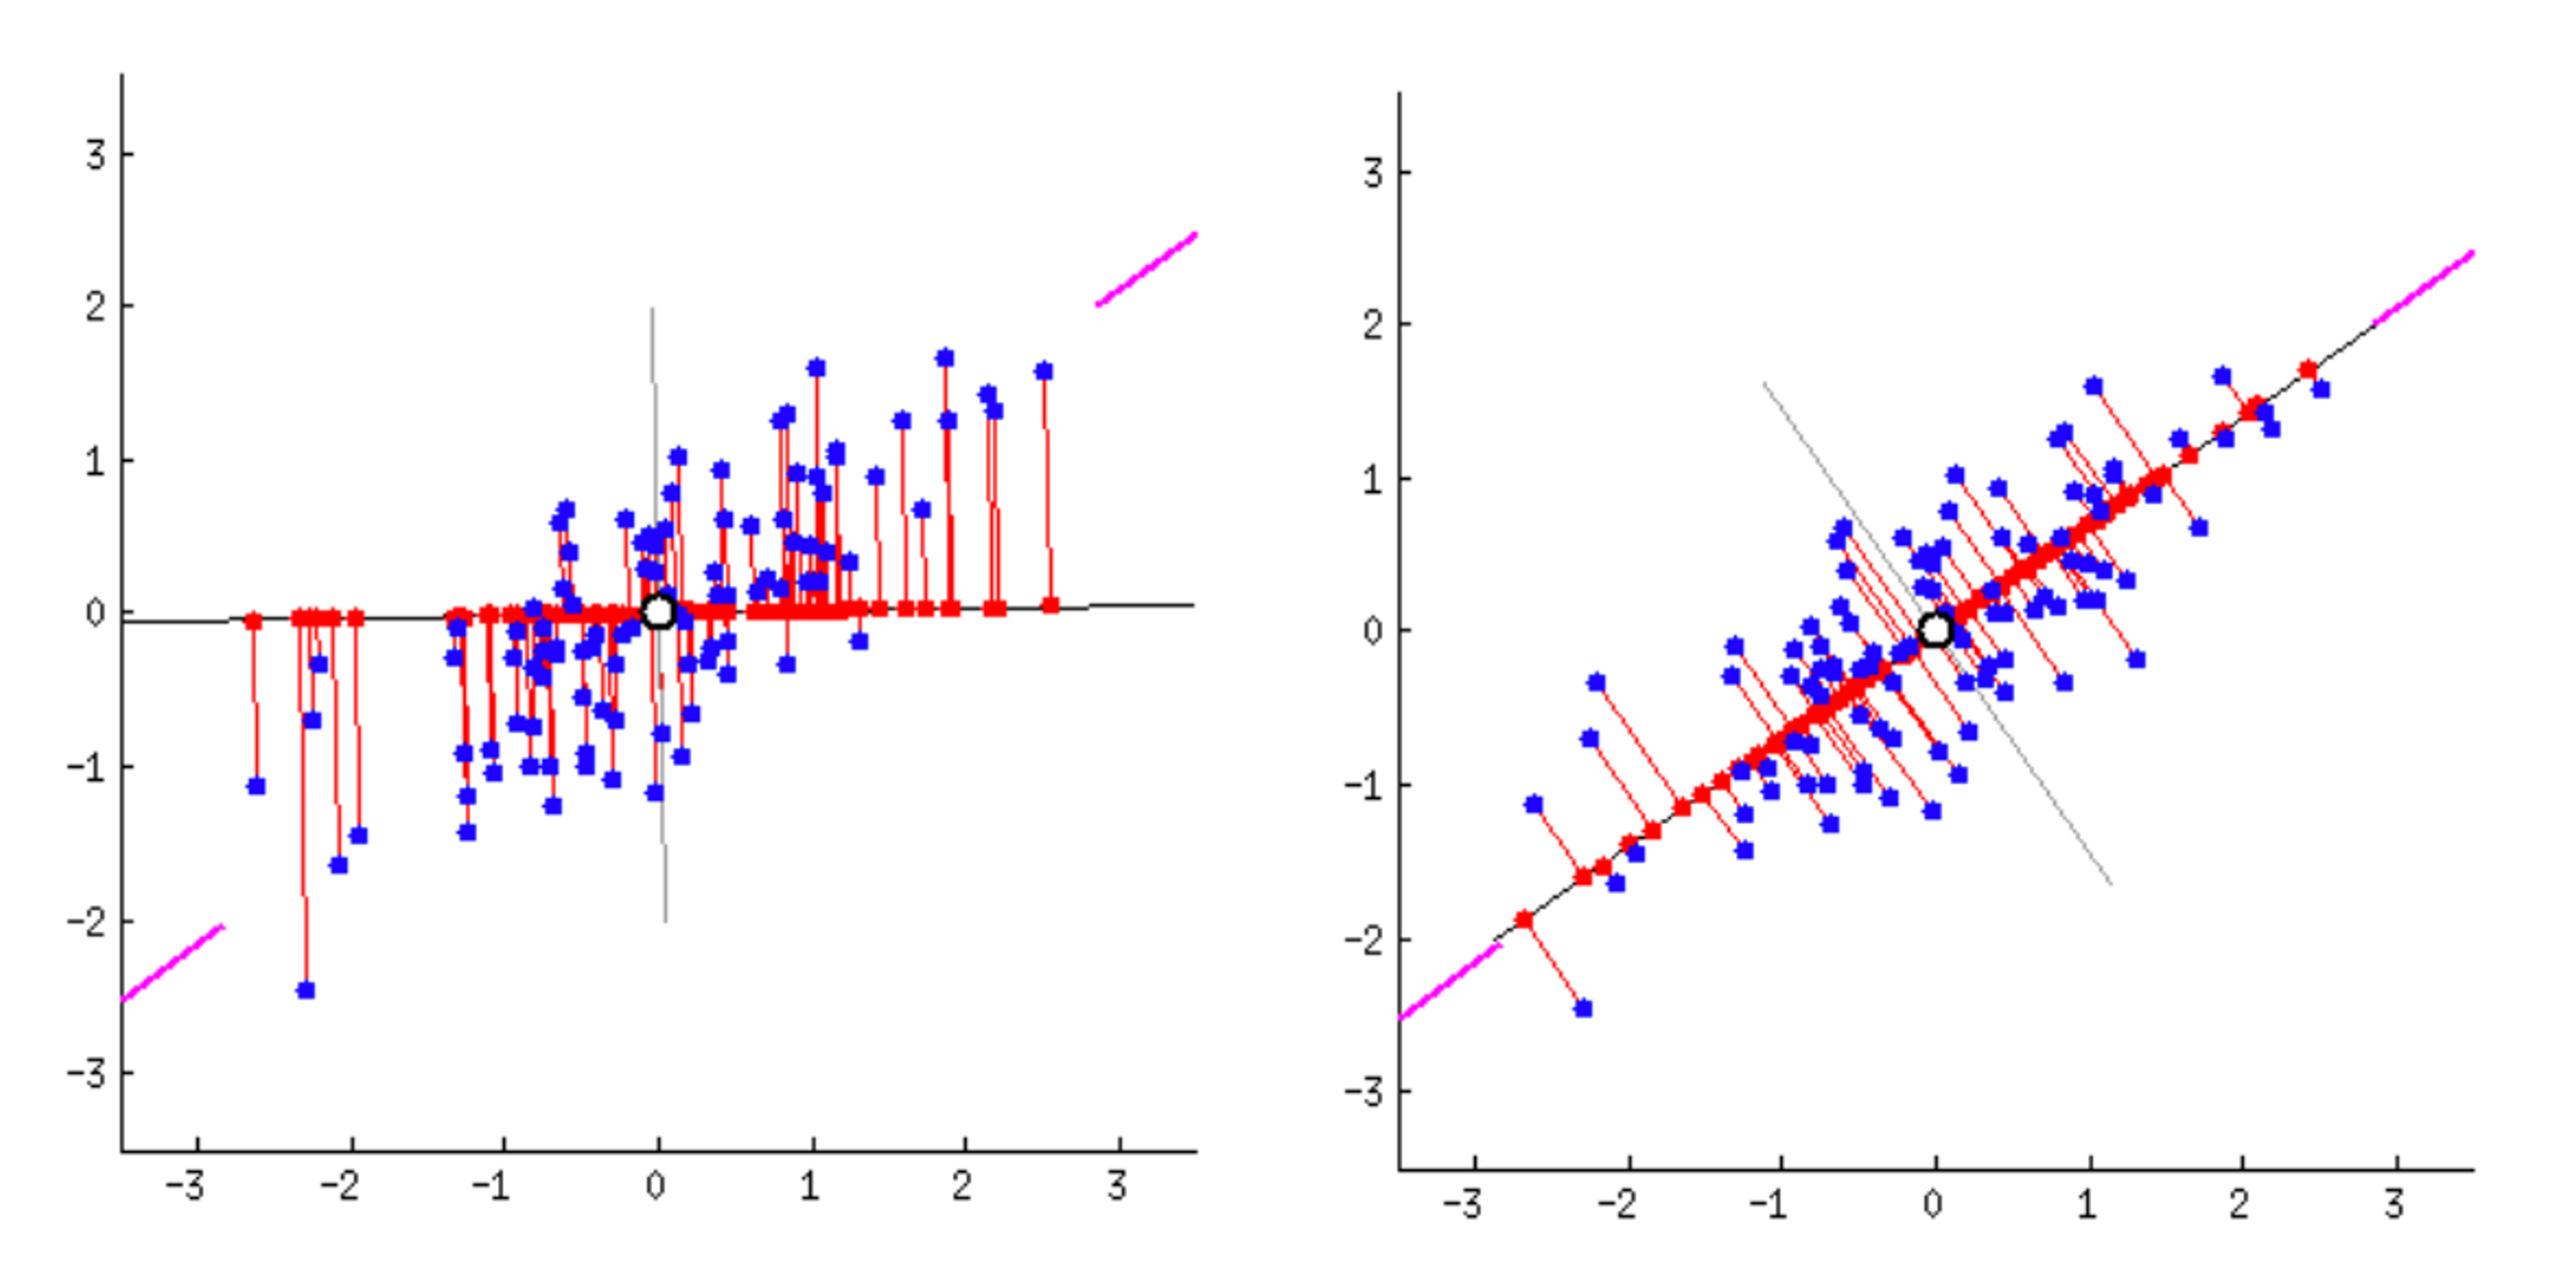
\includegraphics[scale=0.4]{img/PC_2.png}
    \caption{Geometrical interpretation of the first principal component. It accounts for the largest possible variance in the dataset and it represented by the line that matches the purple marks because it goes through the origin and it’s the line in which the projection of the points (red dots) is the most spread out (i.e. maximize the variance) (Ref. \cite{pc}).}
    \label{fig:PC2}
\end{figure}

\textbf{PCA steps} The process to find the principal components can be divided into five steps (Ref. \cite{pc}):

\begin{enumerate}
    \item \textbf{Standardization:} standardize the range of initial variables
    \item \textbf{Correlation matrix}: compute the correlation matrix
    \item \textbf{Eigenvalues and eigenvectors of the correlation matrix:} compute the eigenvalues and eigenvectors of the correlation matrix to identify the principal components
    \item \textbf{Feature vector:} create a feature vector to decide which principal components to keep
    \item \textbf{Recasting:} recast the data along the principal components axes
\end{enumerate}

\textbf{1. Standardization} The aim of this step is making all continuous initial variables equally contributed for the analysis, otherwise if variables range on different scales they lead to biased results.

\begin{equation}
    x = \frac{x -\bar{x}}{\sigma}
\end{equation}
where $\bar{x}$ is the mean value and $\sigma$ is the standard deviation.

\textbf{2. Correlation matrix} In order to reduce the dimensionality of the problem and gather information, a preliminary step is finding correlations among data. The more variables are correlated the more information of the original dataset is redundant. In order to identify these correlations, the correlation matrix needs to be computed (\ref{Morten}):

\scalebox{0.8}{
$$
\boldsymbol{C}[\boldsymbol{x}] = \begin{bmatrix}
1 & \mathrm{corr}[\boldsymbol{x}_0,\boldsymbol{x}_1]  &  \dots & \dots & \mathrm{corr}[\boldsymbol{x}_0,\boldsymbol{x}_{p-1}]\\
\mathrm{corr}[\boldsymbol{x}_1,\boldsymbol{x}_0] & 1  & \dots & \dots & \mathrm{corr}[\boldsymbol{x}_1,\boldsymbol{x}_{p-1}]\\
\mathrm{corr}[\boldsymbol{x}_2,\boldsymbol{x}_0]   & \mathrm{corr}[\boldsymbol{x}_2,\boldsymbol{x}_1] & \dots & \dots & \mathrm{corr}[\boldsymbol{x}_2,\boldsymbol{x}_{p-1}]\\
\dots & \dots & \dots & \dots & \dots \\
\dots & \dots & \dots & \dots & \dots \\
\mathrm{corr}[\boldsymbol{x}_{p-1},\boldsymbol{x}_0]   & \mathrm{corr}[\boldsymbol{x}_{p-1},\boldsymbol{x}_1]  & \dots & \dots  & 1\\
\end{bmatrix}
$$}

where $x$ is the matrix containing all the variables by column, $p$ is the number of variables (or fautures) and 

$$
\mathrm{corr}[\boldsymbol{x},\boldsymbol{y}]=\frac{\mathrm{cov}[\boldsymbol{x},\boldsymbol{y}]}{\sqrt{\mathrm{var}[\boldsymbol{x}] \mathrm{var}[\boldsymbol{y}]}}.
$$

$$
\mathrm{cov}[\boldsymbol{x},\boldsymbol{y}] =\frac{1}{n} \sum_{i=0}^{n-1}(x_i- \overline{x})(y_i- \overline{y}),
$$

$$
\mathrm{var}[\boldsymbol{x}]=\frac{1}{n} \sum_{i=0}^{n-1}(x_i- \overline{x})^2.
$$

Each $\mathrm{corr}[\boldsymbol{x},\boldsymbol{y}]$ spans in $[-1,1]$ and mapping $\boldsymbol{C}[\boldsymbol{x}]$ is then possible to appreciate which variables are more or less correlated, checking higher absolute correlation values or 0 respectively.

\textbf{3. Eigenvalues and eigenvectors of the correlation matrix}
The eigenvectors of the correlation matrix represent the directions of the axes where there is the most variance(i.e. the "principal components"), while the eigenvalues are the coefficients related to each eigenvector, which give the amount of variance carried. By ranking the eigenvectors in order of their eigenvalues, the principal components are then listed in order of significance.

\textbf{4. Feature vector}
The feature vector is simply a matrix that has as columns the eigenvectors of the components that we decide to keep and has as feutures dimension $l < p$ (i.e. dimensionality reduction).

\textbf{5. Recasting}
In the previous steps, the selection of the principal components is done, but the input data set remains always in terms of the original axes (i.e, in terms of the initial variables). In order to reorient the data from the original axes to the new ones, it simply needs to multiplying the transpose of the original data $X^{T}$ set by the transpose of the feature vector $V^{T}$:

\begin{equation}
    X^{*} = X^{T} * V^{T}
\end{equation}

An important point to underline is that this method is more effective (i.e. least number of PC) when the data are highly correlated, so the very first principal components gather the far majority of the information (i.e. variance, Figure \ref{fig:PC}). If this doesn't happen, another way of seeing the problem is choosing the number of the PC according to the total variance is wished to be covered (e.g. first 4 components account for the 95\% of the variance) (Ref. \cite{pc2}).

\subsection{Logistic Regression}
Logistic regression is a class of regression analysis where the output is dichotomous (binary) or multicategorical, which cannot be modelled with a linear method (Ref. \cite{log1}). Linear regression gives a continuous output, while logistic regression provides a constant output. This is why the continuous function $f(x)$ that models the linear outcome turns into a probability distribution $p(x)$ in logistic regression, as shown in Figure \ref{fig:log}. The choice of the probability function is arbitrary, but the most common one is the \textit{sigmoid} function, often called "logistic function" indeed:
$$
p(x) = \frac{1}{1 + e^{-x}},
$$
The Logistic regression is one of the most simple and commonly used Machine Learning algorithms and its basic fundamental concepts are constructive in deep learning (Ref. \cite{log2}).

\begin{figure}[h]
    \centering 
    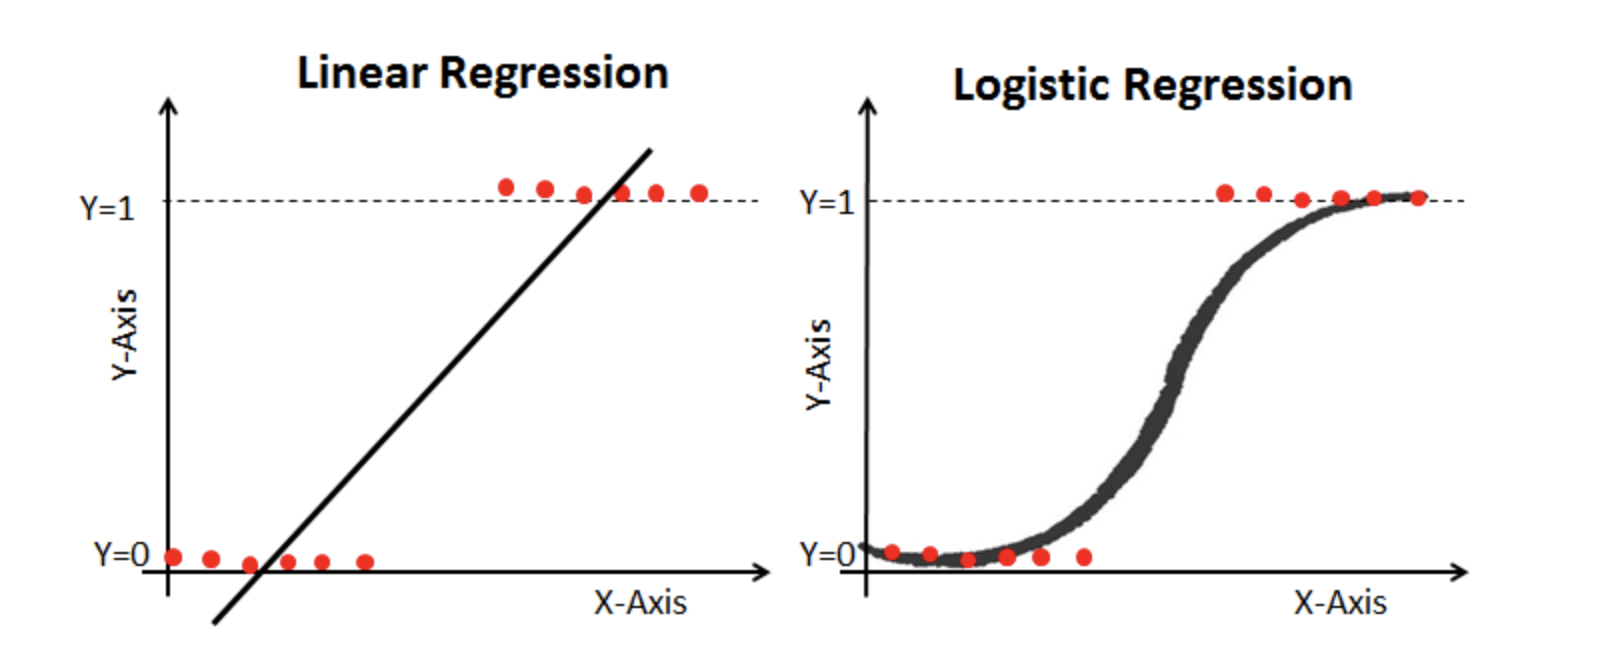
\includegraphics[scale=0.3]{img/Logistic_Regr.png}
    \caption{Limitations of Linear Regression in modelling binary output versus a qualitative sigmoid function fitting properly the data (Ref. \cite{log2}).}
    \label{fig:log}
\end{figure}

\subsection{Deep Neural Network}

The basic idea of Deep Neural Network lies on building a system of interconnected units, called \textit{neurons}, divided in multiple layers, that broadcast signals throughout the neural system. The structure is composed of an input layer, one or more hidden layers, with different number of neurons in each of them, and the output layer. The broadcasting of the signal happens thanks to \textit{activation functions} that elaborate the input signals for each neuron into the ouput ones. They are coupled with weights and biases associated to each neuron so that the output is more or less relevant when broadcasted to the next layer (Figure \ref{fig:nn}). This process starts from the input layer and it runs thoughtout each neuron of each layer, until resulting into an output layer, that is the model prediction (i.e.\textit{Feed Forward Neural Network}). The next step is to \textit{train} the network. Given already the expected \textit{true} output, it is compared to the model prediction thanks to a \textit{cost function} that evaluates the performance of the model. The aim is to minimize this value and using the \textit{backpropagation} and Stochastic Gradient Descent (SGD) algorithms, is possibile to optimize the parameters (i.e. weights and biases) to have the closest result to the expected one. This last step is extremely important because then the network is able to \textit{predict} the results given any other input data. The overall performance of the network is evaluated thanks to the \textit{metrics} on a test dataset (Ref. \cite{mortens}). For any further information about FFNN, backpropagation algorithm, activation functions, SGD optimizers, cost  functions, metrics look at the previous report "Report 2: Feed Forward Neural Network" \cite{adele}, where information has already been summarized and gathered.

\begin{figure}[h]
    \centering 
    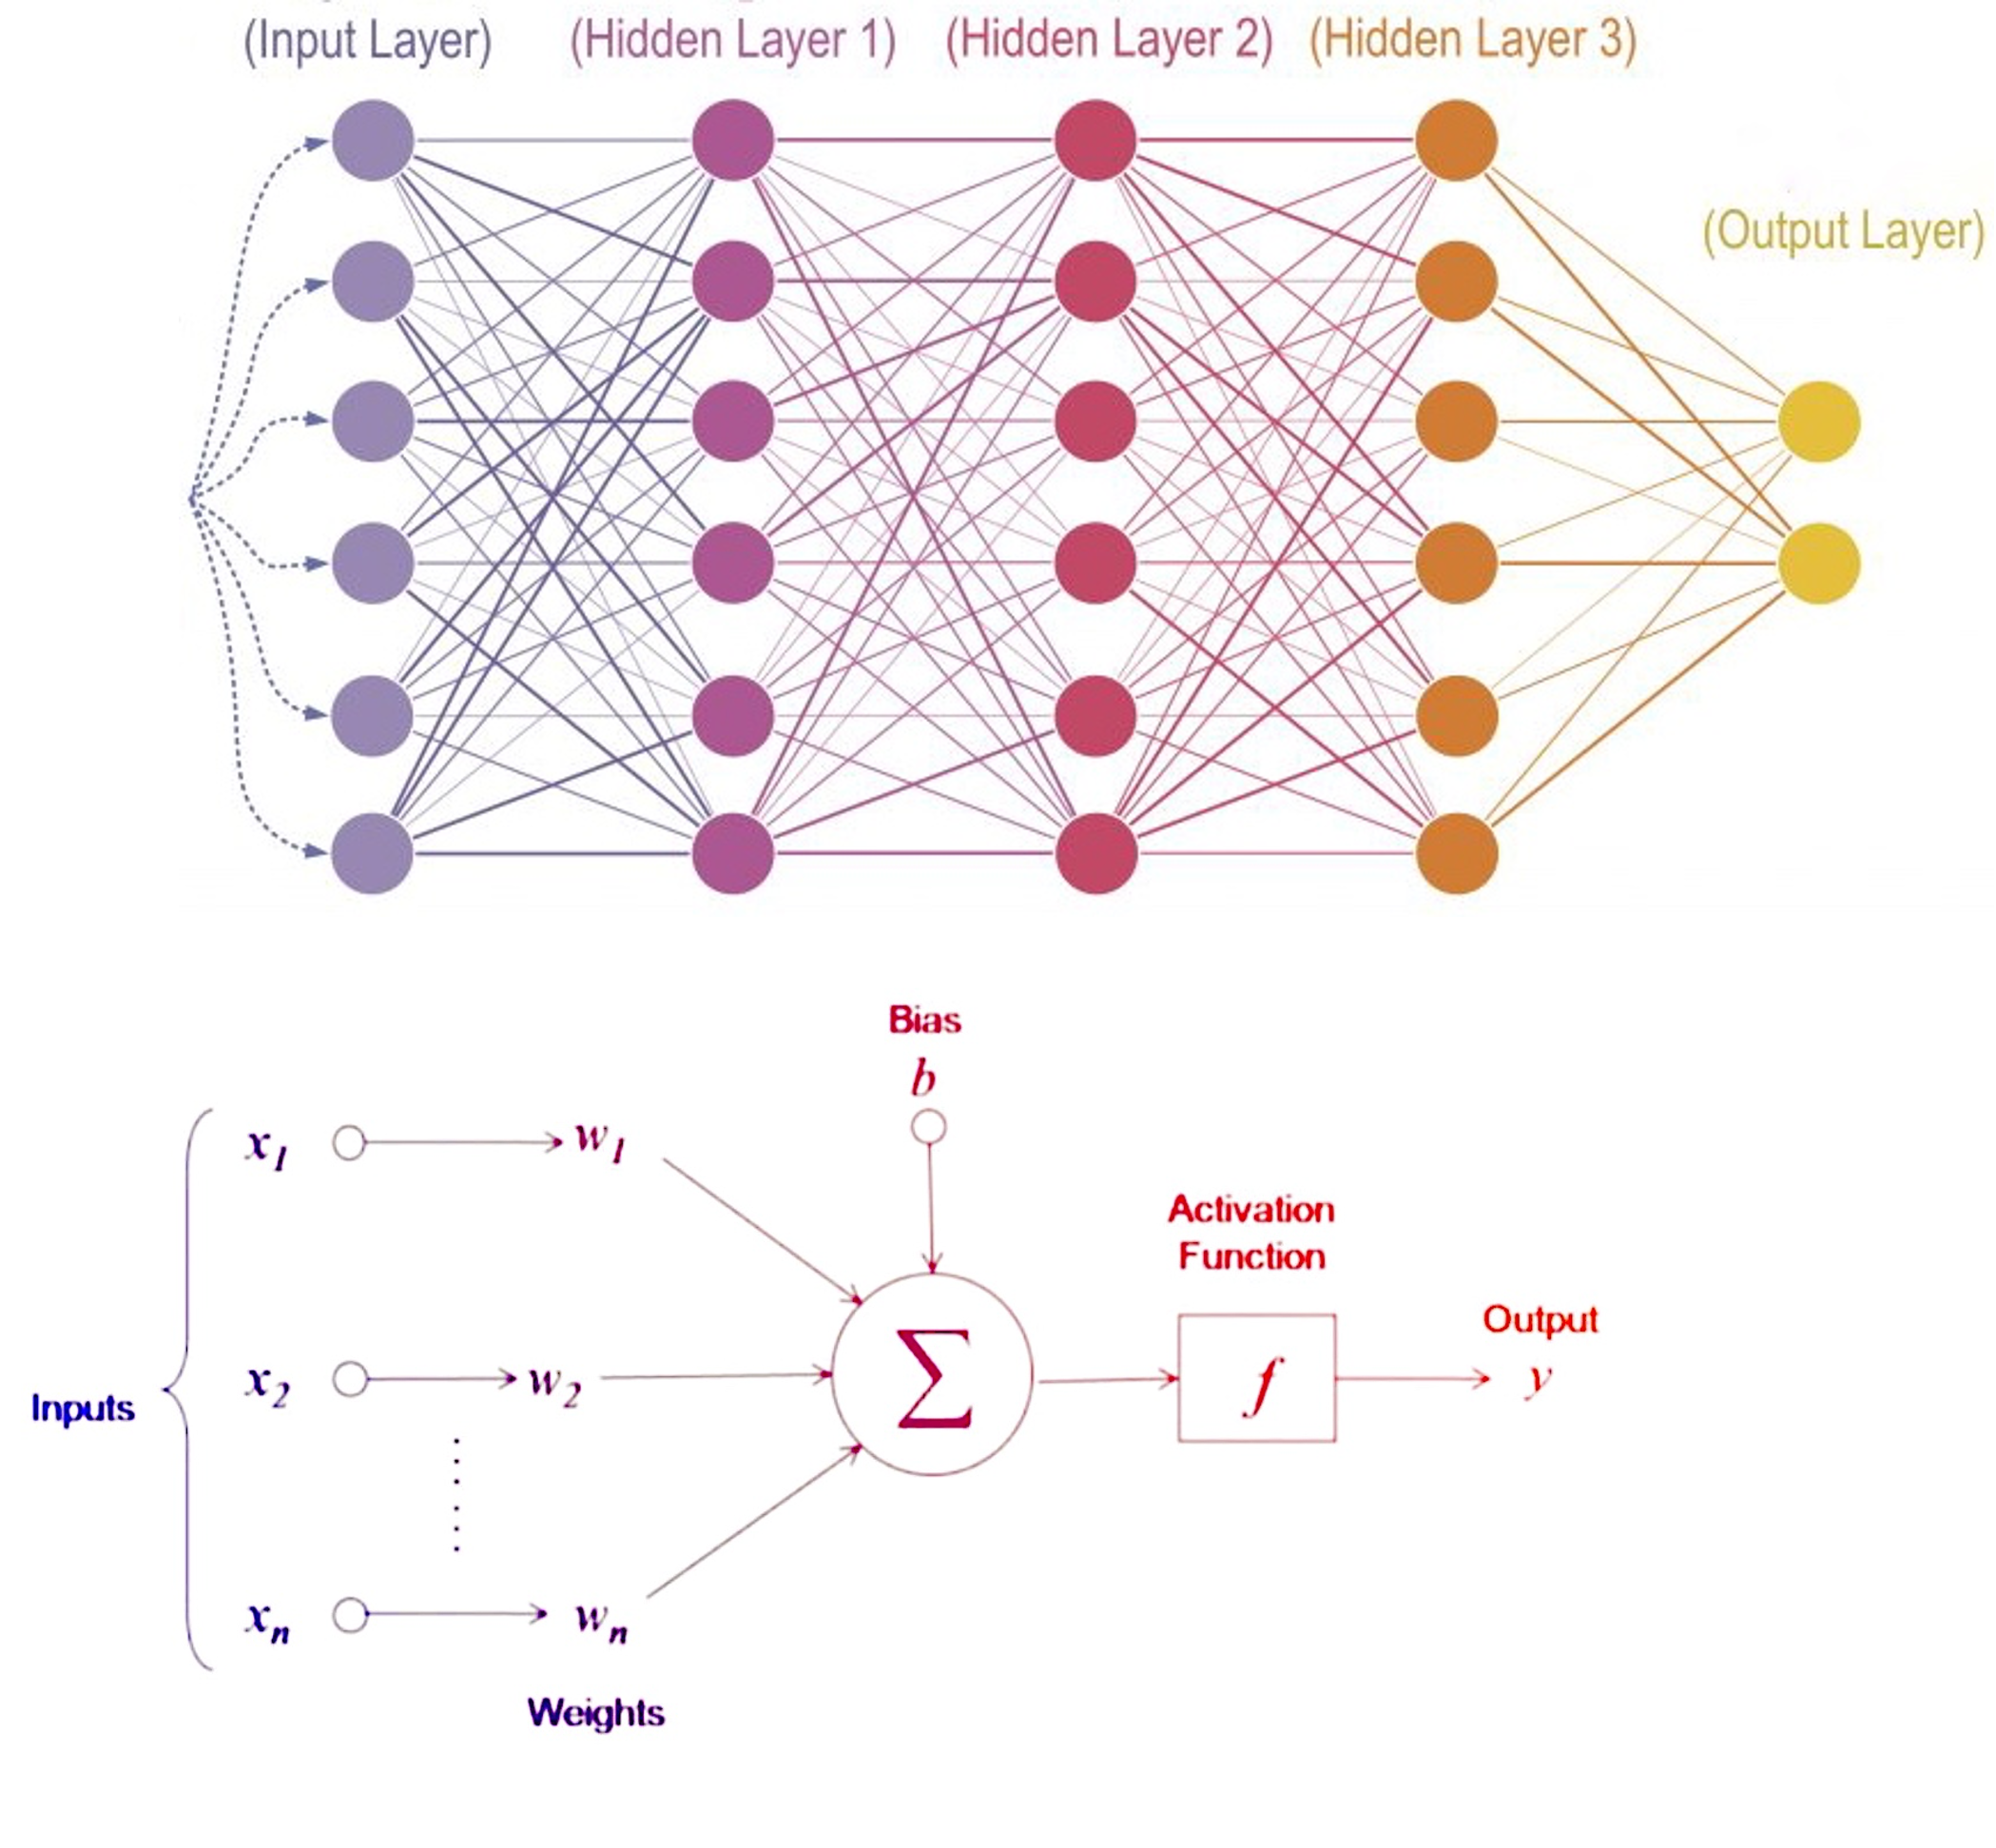
\includegraphics[scale=0.5]{img/neural_network_structure.png}
    \caption{Examples of Neural Network architecture, with several neurons divided into the hidden layers and with a focus on one single neuron and its schematic operation.}
    \label{fig:nn}
\end{figure}

\subsection{Support Vector Machine}
The Support Vector Machine (SVM) is another supervised learning technique, used for both regression and classification problems, even though it is mainly known for classification (SMC). Unlike most algorithms, SVM makes use of a hyperplane which acts as a decision boundary between the various classes. The optimal hyperplane is the one that has the maximum distance, called margins, from the closest datapoints from each class, known as Support Vectors \cite{svm3}. The basic idea is shown in Figure \ref{fig:svm}.
 
 \begin{figure}[h]
    \centering 
    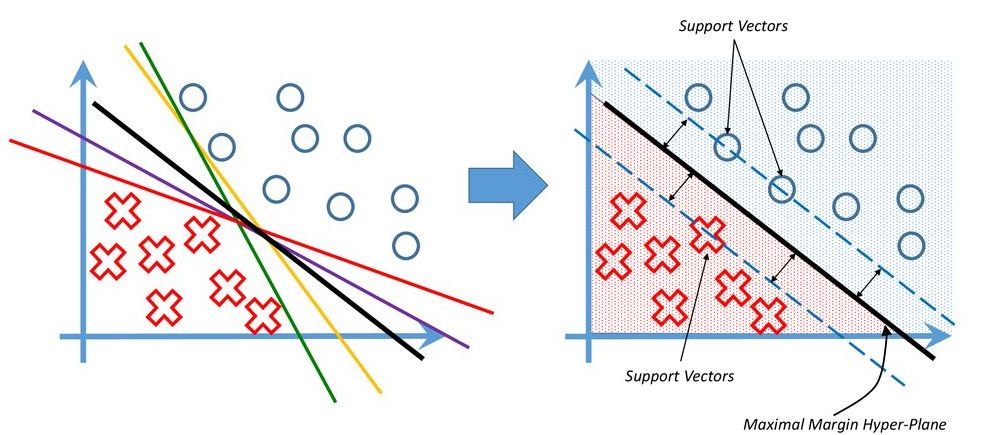
\includegraphics[scale=0.2]{img/Support_Vector_Machines.jpg}
    \caption{Schematic idea of the optimal hyperplane in SVM (Ref. \cite{svm2})}
    \label{fig:svm}
\end{figure}

 
 
The SVM can also be used for classifying non-linear type of data using kernels, such as Linear, RBF, Sigmoid, Poly. These kernels are used in transforming the non-linear data into an high dimensional feature space, in this way an hyperplane will be created between various classes of non-linear data (Ref. \cite{svm3}, \cite{svm4}), as shown in Figure \ref{fig:kernel}. For any further information on this topic check Ref. \cite{svm1}.

 \begin{figure}[h]
    \centering 
    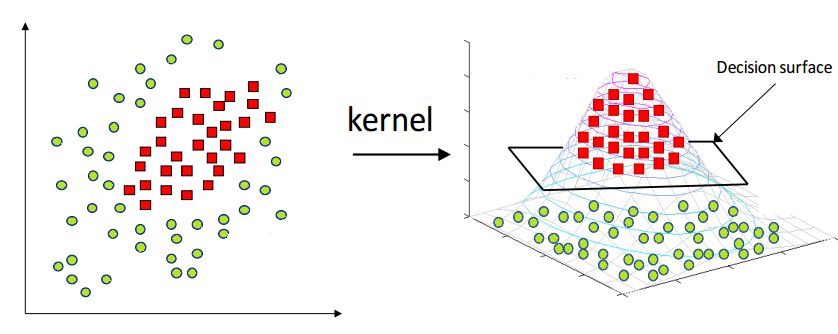
\includegraphics[scale=0.25]{img/kernel.png}
    \caption{The kernel trick that transforms the input space into a higher dimensional space, called the feature space, where a linear separation can be performed (Ref. \cite{svm1}).}
    \label{fig:kernel}
\end{figure}



\section{Methods} \label{sec:methods}

This work aims to evaluate and compare the performance of three Machine Learning techniques. As a classification problem is here analysed, the accurancy score, the confusion matrix and the ROC metric are employed to quantify the performance. This section will first present the code implementation of each Machine Learning technique together with the metrics used to evaluate the performance of the models. 


% ===========================================
\subsection{Code implementation}\label{sec:code}

During the previous projects, we implemented our own codes to solve the problems, while in the present work, my intention is to explore and use the Scikit-Learn \cite{sk} and Tensorflow \cite{tf} packages. The reasons rely on the practical use of the Machine Learning techniques I will have after this course: these packages offer a wide range of ML methods with several functionalities, the code is very versatile and it has been widely used and tested, compared to the one that I made for the previous projects that is made from scratch and the quality is much lower. I take here the opportunity to explore and master these packages better for my future utilization. Another reason is about the conclusions I have taken from the previous projects: the far majority of the time and energy was employed in implementing the code and especially in solving computational problems, while very little time was left for the proper analysis of the performance. I learnt a lot from the previous projects and in spite of my passion for coding in this work I would like to concentrate on something new.

In order to perform the PCA as described in Section \ref{sec:pc}, the \texttt{PCA} method from Scikit-Learn has been applied, but instead of specifying the number of principal components, $n\_components$ is set to be a float between 0.0 and 1.0, indicating the ratio of variance to preserve. For the ML models \texttt{LogisticRegression} and \texttt{SVC} has been used from the Scikit-Learn package for the Logistic Regression and Classifier Support Vector Machine respectively, while for building the Neural Network the functionalities in Keras \cite{keras} has been applied. For further details, the source code can be found on GitHub in the \href{https://github.com/adelezaini/MachineLearning/tree/master/Projects/Project3}{Machine Learning} repository.

%The kernel PCA has been choosen because it includes nonlinearity in the very high-dimensional space of features, that makes it very suitable when dealing with Support Vector Machines. It is a mathematical technique that implicitly maps instances into a very high-dimensional space, enabling complex nonlinear classification and regression projections for dimensionality reduction. For further information check Ref. \cite{mortens}  and \ref{ref:wiki_kPCA}).

\subsection{Metrics}

In order to evaluate and compare the performance of the three techniques, the accuracy score, the confusion matrix and the ROC curve are the chosen metrics. Before going into the definition of these metrics, we define some classification parameters (Ref. \cite{classpar}), common to the three metrics :

\begin{itemize}
    \item[-] \textbf{TP - True Positive}: outcome where the model correctly predicts the positive class;
    \item[-] \textbf{TN - True Negative}: outcome where the model correctly predicts the negative class
    \item[-] \textbf{FP - False Positive}: outcome where the model incorrectly predicts the positive class
    \item[-] \textbf{FN - False Negative}: outcome where the model incorrectly predicts the negative class.
    \item[-] \textbf{TPR - True Positive Rate}: 
    $$TPR = TP / (TP+FN)$$
    \item[-] \textbf{FPR - False Positive Rate}: 
    $$FPR = FP / (FP+TN)$$
\end{itemize}

\textbf{Accuracy score}
$$
\text{Accuracy} = \frac{\sum_{i=1}^n I(t_i = y_i)}{n} ,
$$

Here $t_i$ represents the target, $y_i$ the outputs of the model, $n$ is the number of targets $t_i$ and $I$ is the indicator function: $1$ if $t_i = y_i$ and $0$
otherwise (Ref. \cite{mortens}).

\textbf{Confusion matrix}
A confusion matrix is a technique for evaluating the performance of a classification algorithm, where the number of correct and incorrect predictions are summarized. This technique can give more insights than the accuracy score, especially when there is unequal number of observations in each class (Ref. \cite{cfm}). The Figure \ref{fig:confmatr} shows the structure of the confusion matrix.

 \begin{figure}[h]
    \centering 
    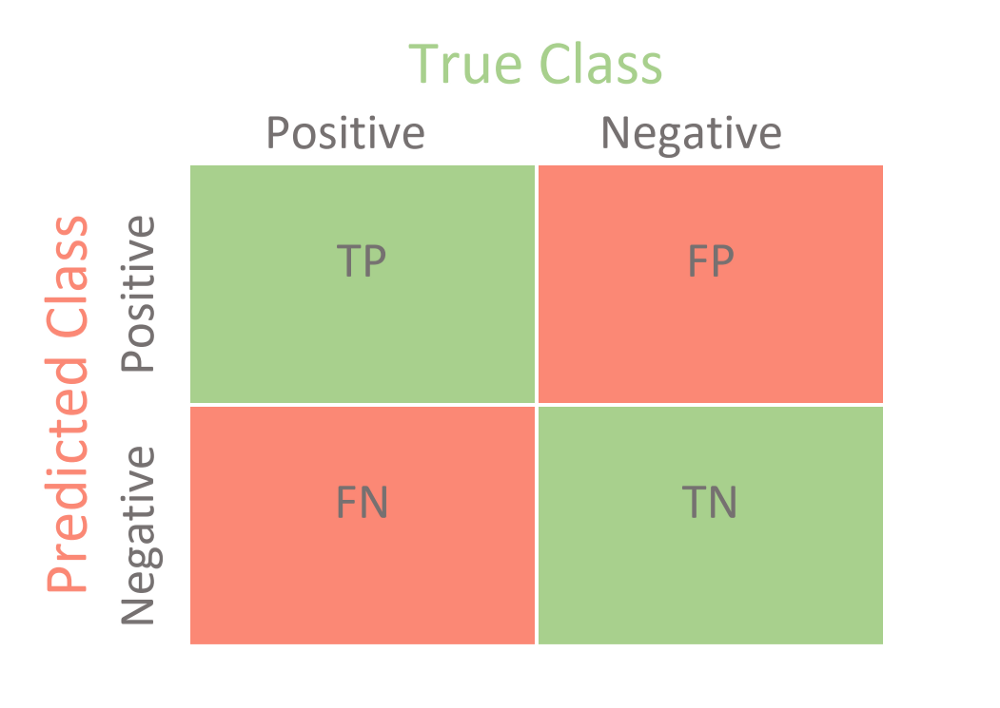
\includegraphics[scale=0.2]{img/confusion_matrix.png}
    \caption{Typical structure of the confusion matrix on a binary classification problem (Ref. \cite{cfm_fig})}
    \label{fig:confmatr}
\end{figure}


\textbf{ROC curve} An ROC curve (receiver operating characteristic curve) is a graph showing the performance of a classification model at all classification thresholds. This curve plots the TPR on the x-axes and the FPR on the y-axes (Ref. \cite{mortens}, \cite{roc}). The ideal curve is a sharp 90° angle as shown in Figure \ref{fig:roc}.

 \begin{figure}[h]
    \centering 
    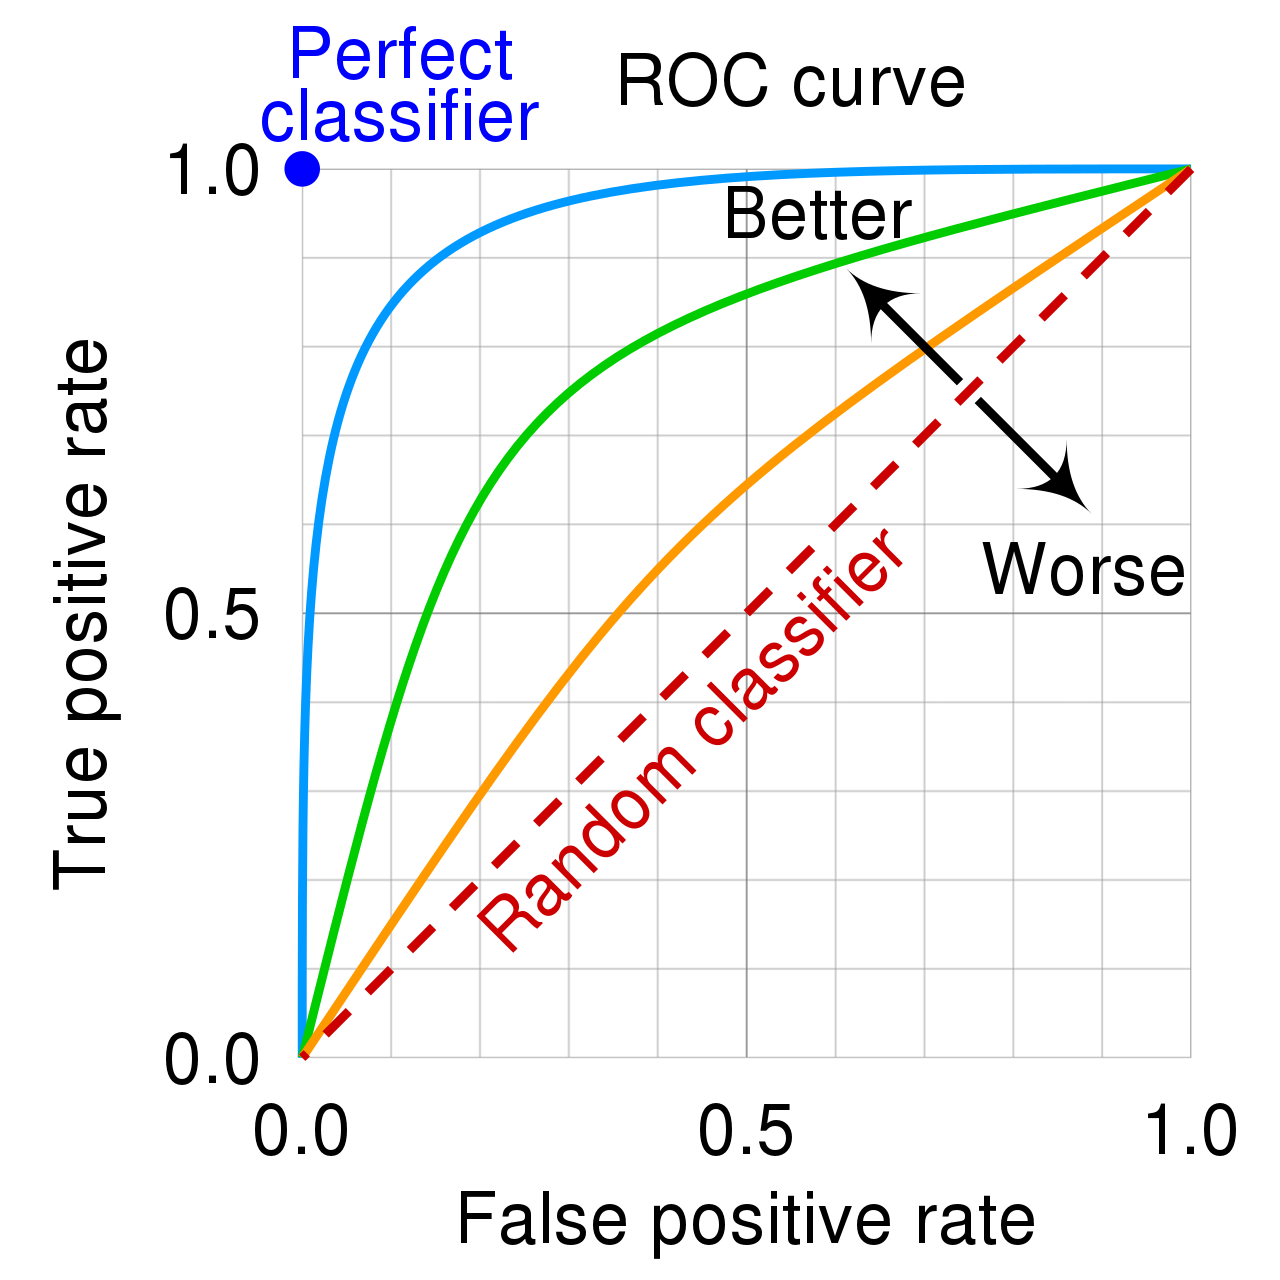
\includegraphics[scale=0.15]{img/Roc_curve.png}
    \caption{ROC curves showing performance of different classifiers (Ref. \cite{roc_fig})}
    \label{fig:roc}
\end{figure}

In order to implement these metrics the methods \textttt{score}, \textttt{confusion\_matrix}, \textttt{roc\_curve} have been used from the Scikit-Learn package. All the source code can be found on GitHub in the \href{https://github.com/adelezaini/MachineLearning/tree/master/Projects/Project3}{Machine Learning} repository.


% ===========================================
\section{Results and discussion}\label{sec:results}

As mentioned in Section \ref{sec:data}, a preliminary analysis has been performed on the original dataset. A dimension reduction was tried, applying the Principal Component Analysis taken as cumulative variance 95\%, 70\%, 55\%, giving respective number of components: 18, 13, 10. This led to the trade off of choosing between reducing the number of features loosing lots of information or keeping information but also the high number of dimensions. Since this is not an extreme case in which we loose so much of the computer efficiency, keeping all the 18 features resulted to be the choice and the following analysis was performed on a training dataset of dimension (360, 18), i.e. Study 1 and 2, and a test dataset of dimension (180, 18), i.e. Study 3.

\begin{figure}[h]
    \centering 
    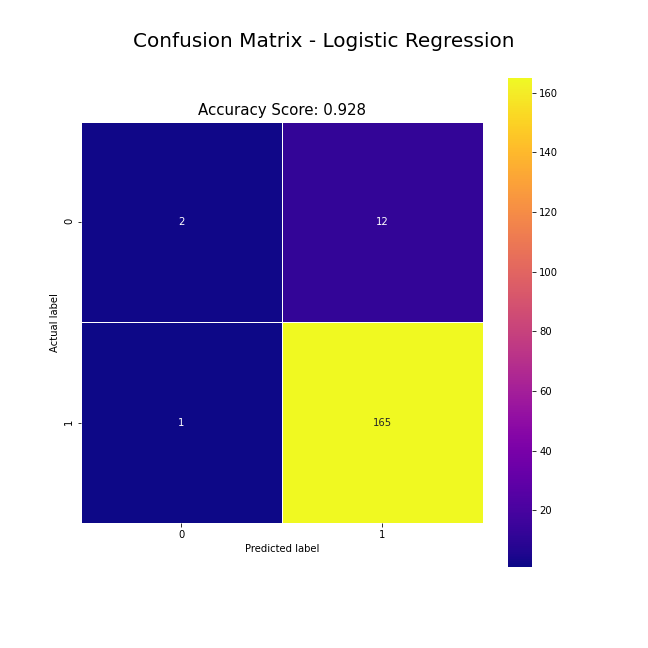
\includegraphics[scale=0.3]{results/confusionmatrix_logreg.png}
    \caption{Confusion matrix of the Logistic Regression. The upper left cell indicates the True Positives (TP) that are the right predicted failures, the upper right represents the False Negatives (FN) that are the missed failures, the bottom left is the False Positive (FP) that stands for the incorrectly predicted failures and the bottom right that are the right predicted success or True Negative (TN).}
    \label{res:cm_log}
\end{figure}

\begin{figure}[h]
    \centering 
    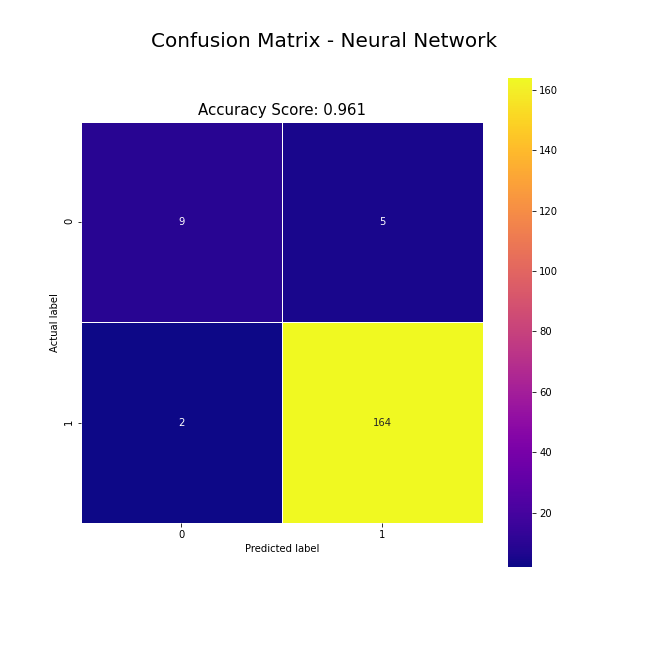
\includegraphics[scale=0.3]{results/confusionmatrix_nn.png}
    \caption{Confusion matrix of the Neural Network. The upper left cell indicates the True Positives (TP) that are the right predicted failures, the upper right represents the False Negatives (FN) that are the missed failures, the bottom left is the False Positive (FP) that stands for the incorrectly predicted failures and the bottom right that are the right predicted success or True Negative (TN).}
    \label{res:cf_nn}
\end{figure}
\begin{figure}[h]
    \centering 
    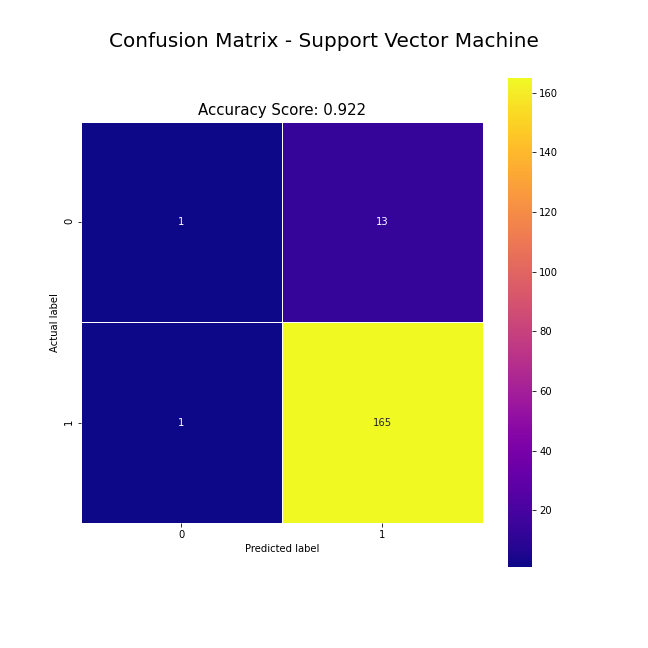
\includegraphics[scale=0.3]{results/confusionmatrix_svm.png}
    \caption{Confusion matrix of the Support Vector Machine. The upper left cell indicates the True Positives (TP) that are the right predicted failures, the upper right represents the False Negatives (FN) that are the missed failures, the bottom left is the False Positive (FP) that stands for the incorrectly predicted failures and the bottom right that are the right predicted success or True Negative (TN).}
    \label{res:cf_svm}
\end{figure}
\begin{figure}[h]
    \centering 
    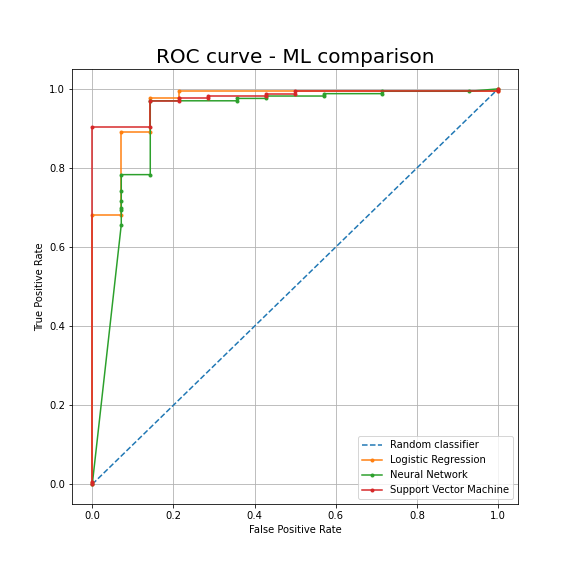
\includegraphics[scale=0.3]{results/ROC_comp.png}
    \caption{ROC curves by comparison for the LR (orange), NN (green) and SVM (red).}
    \label{res:roc}
\end{figure}

For the Logistic Regression (LR) and SVM default parameters are chosen, the Neural Network (NN) is composed by three hidden layers with the \textit{ReLU} as activation function and \textit{Adam} as optimizer (look at the previous report for further details on these parameters \cite{adele}). In order to compare the performance of the three models, we refer to the accuracy scores and confusion matrices in Figures \ref{res:cm_log}, \ref{res:cf_nn}, \ref{res:cf_svm}, while the ROC comparison is shown in Figure \ref{res:roc}. The accuracy scores for the LR, for the NN and for the SVM are respectively of $92.8\%$, $96.1\%$, $92.2\%$, meaning that all the three models perform very well in the overall performance. Nevertheless, if we have closer look at the confusion matrices, we can actually see that they basically predict very few failures of the climate simulations: $2$ for LR, $9$ for NN, $1$ for SVM, when the real number expected was $14$. Note that TP (upper left) stands for actual failures, FN (upper right) stands for missed failures and so on. This behaviour is understandable because the test sample is quite small combined with the fact that there is a very high inequality in the number of failures and successes in the already small sample. We are comparing something that relatively speaking leads to a big error (e.g. for LR $|2-14|/14=85\%$), but speaking in absolute terms there is little distance compared to the whole sample (e.g. for LR $|2-14|/180=7\%$). This is why the accuracy score in very high in the three models, shown also by the ROC curve, where all the three models are very close to the ideal sharp curve (Figure \ref{fig:roc}). Going back to the objective of this analysis though, this is using ML techniques to predict the simulations failures. This then mean that the only model that reaches a close result is the NN, while the other two fail in this goal. The reasons why the NN perfoms better than the LR are that the first is a very more sofisticated techinque than the latter. As SVM is concerned, the result is instead quite surprising, because this technique would be eligible for high dimensional spaces, as it is in the present case (Ref. \cite{svm5}). Further investigations need to be conducted.

\begin{table}[]
\begin{tabular}{ccccc}
\hline
\multicolumn{5}{c}{Activation functions VS Optimizers}                                                     \\ \hline
                                      & \textit{sgd} & \textit{adagrad} & \textit{rmsprop} & \textit{adam} \\ \cline{2-5} 
\multicolumn{1}{c|}{\textit{relu}}    & 0.961        & 0.961            & 0.967            & 0.967         \\
\multicolumn{1}{c|}{\textit{sigmoid}} & 0.922        & 0.978            & 0.972            & 0.961         \\
\multicolumn{1}{c|}{\textit{tanh}}    & 0.967        & 0.967            & 0.950            & 0.950         \\
\multicolumn{1}{c|}{\textit{elu}}     & 0.978        & 0.956            & 0.878            & 0.961        
\end{tabular}
\caption{Accuracy scores of Neural Networks with different activation functions and optimizers.}
\label{tab:nn}
\end{table}

\begin{figure}[h]
    \centering 
    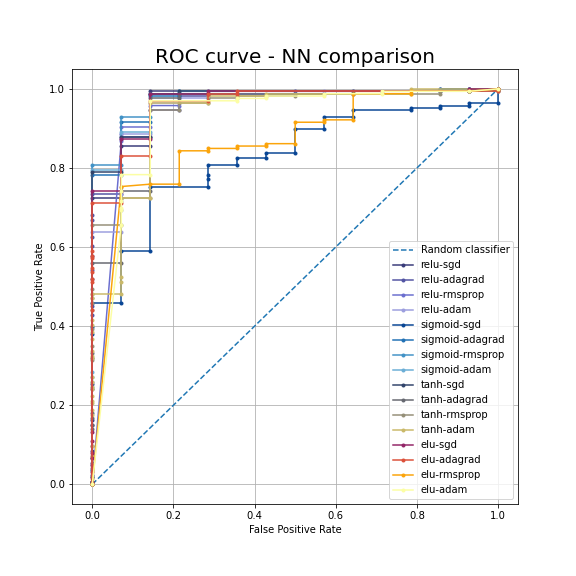
\includegraphics[scale=0.3]{results/ROC_comp_NN.png}
    \caption{ROC curves for different NN, changing the activation functions (\textit{'relu', 'sigmoid','tanh','elu'}) and the optimizers \textit{'sgd', 'adagrad','rmsprop','adam'}).}
    \label{res:roc_nn}
\end{figure}

The second step of the analysis involves "optimizing" the NN, i.e. comparing the performance of the NNs setting different activation functions and optimizers. We can see from Table \ref{tab:nn} that all the accuracy scores are very high and so the ROC curves are all sharp (Figure \ref{res:roc_nn}). Nevertheless, we can also notice little differences. What in every run of the code is constant is the worst performance of the combinations \textit{'elu-adagrad'} and \textit{'sigmoid-sgd'}, which have respectively $87.8\%$ and $92.2\%$ of accuracy scores and are the ones' curves that evidently perform worst in the ROC plot. It is hard to choose an eligible best combination, because lots of them perform very similarly. Even running the code several times, the best one keep changing, but the \textit{'elu-sgd'} is always on the top of the ranking. The reasons behind these behaviours are not completely clear but this grid analysis was needed to have further insights on the NN optimal parameters perhaps for future research. In the Appendix all the confusion matrices are collected in Figure \ref{res:nn_tot}.

% ===========================================
\section{Conclusions and outlook}\label{sec:conclusion}

In this report we explored different Machine Learning techniques (Logistic Regression, Deep Neural Network and Support Vector Machine) by comparison in performing a classification problem on the UCI dataset Climate Model Simulation Crashes \cite{UCI}. The evaluation of the performance was done by evaluating the accuracy score, the confusion matrix and the ROC curve. For the first and last metrics all the three models seem to have an excellent behaviour but looking into the confusion matrices, it is possible to appreciate that only the Neural Network succeed in predicting when the simulations crashes could happen. An optimization of the Neural Network has been carried out, varying the activation functions and the optimizers. For several combinations, the networks perform very well, except for \textit{'elu-adagrad'} and \textit{'sigmoid-sgd'}.

The work underlying this report was aiming to compare the Machine Learning techniques, but reading the Lucas D.D. et al.'s study \cite{failure} other ideas out of the report objectives can be explored in further investigations, such as the sensitivity analysis, reproducing for instance Figure \ref{data:sens}). In addition, during this work default parameters of the Sklearn's methods have been considered. exploring the parameters' space would be very interesting in future studies.

\onecolumngrid

\clearpage
\section*{Appendix}\label{sec:appendix}
\begin{figure}[h]
    \centering 
    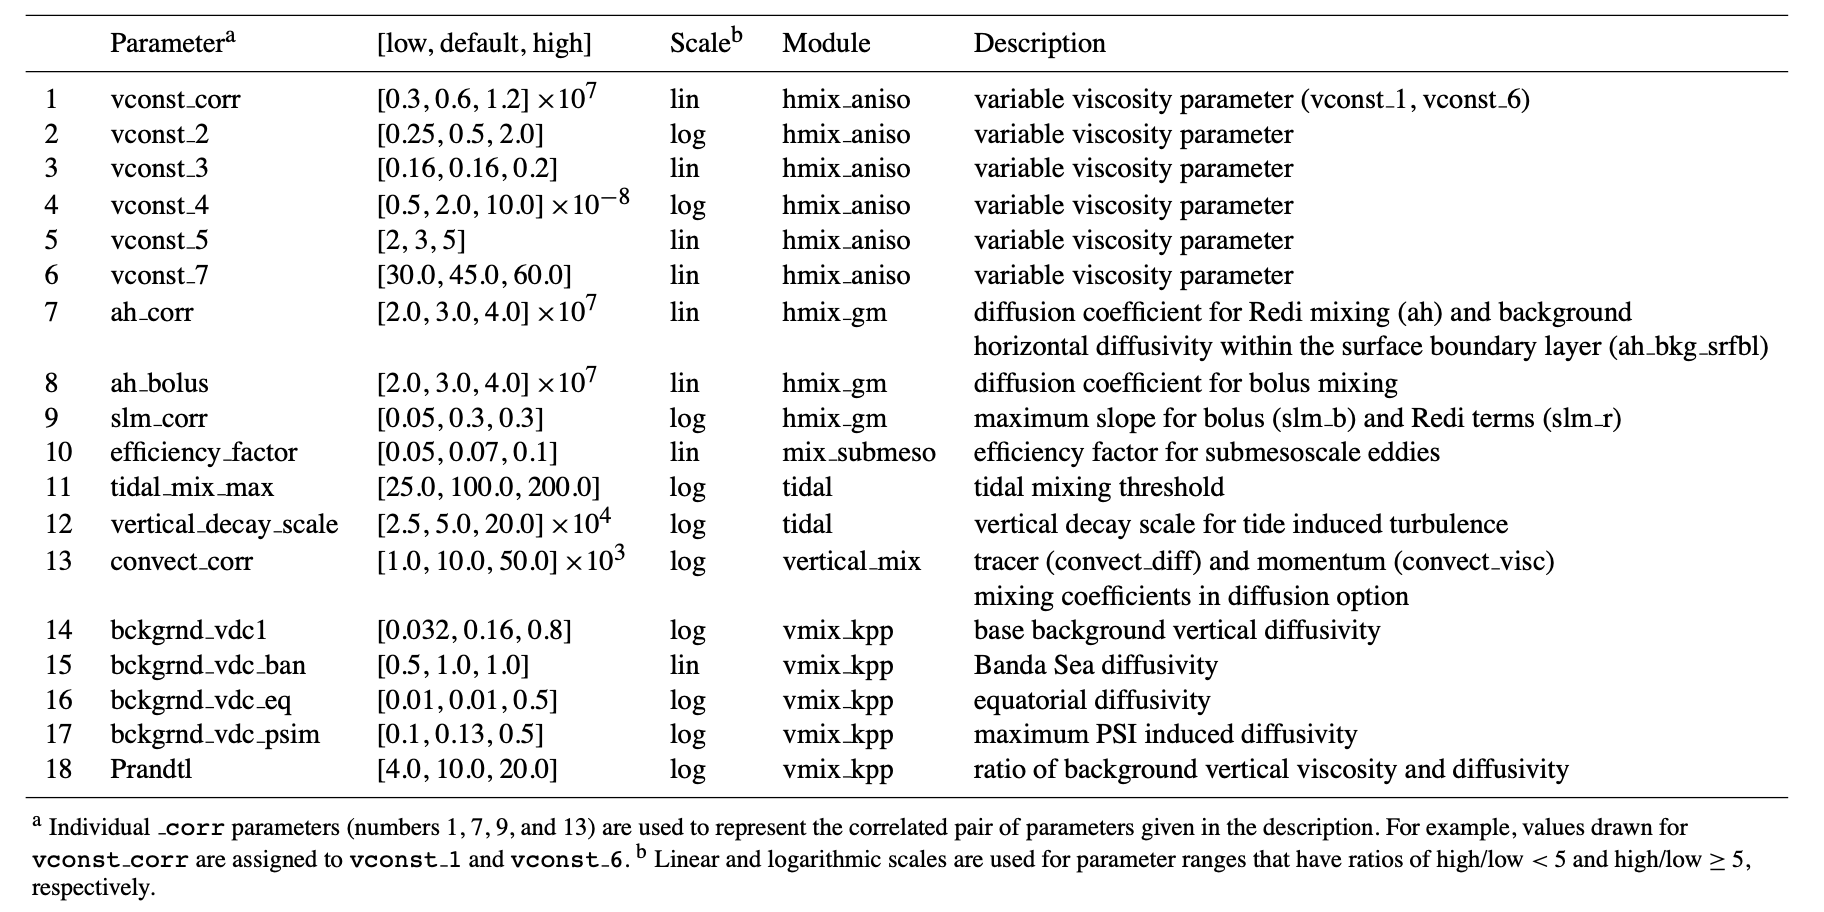
\includegraphics[scale=0.5]{img/big_big_table.png}
    \caption{Complete description of the 18 features (Ref. \cite{failure})}
    \label{fig:big_big_table}
\end{figure}

\begin{figure}[h]
    \centering 
    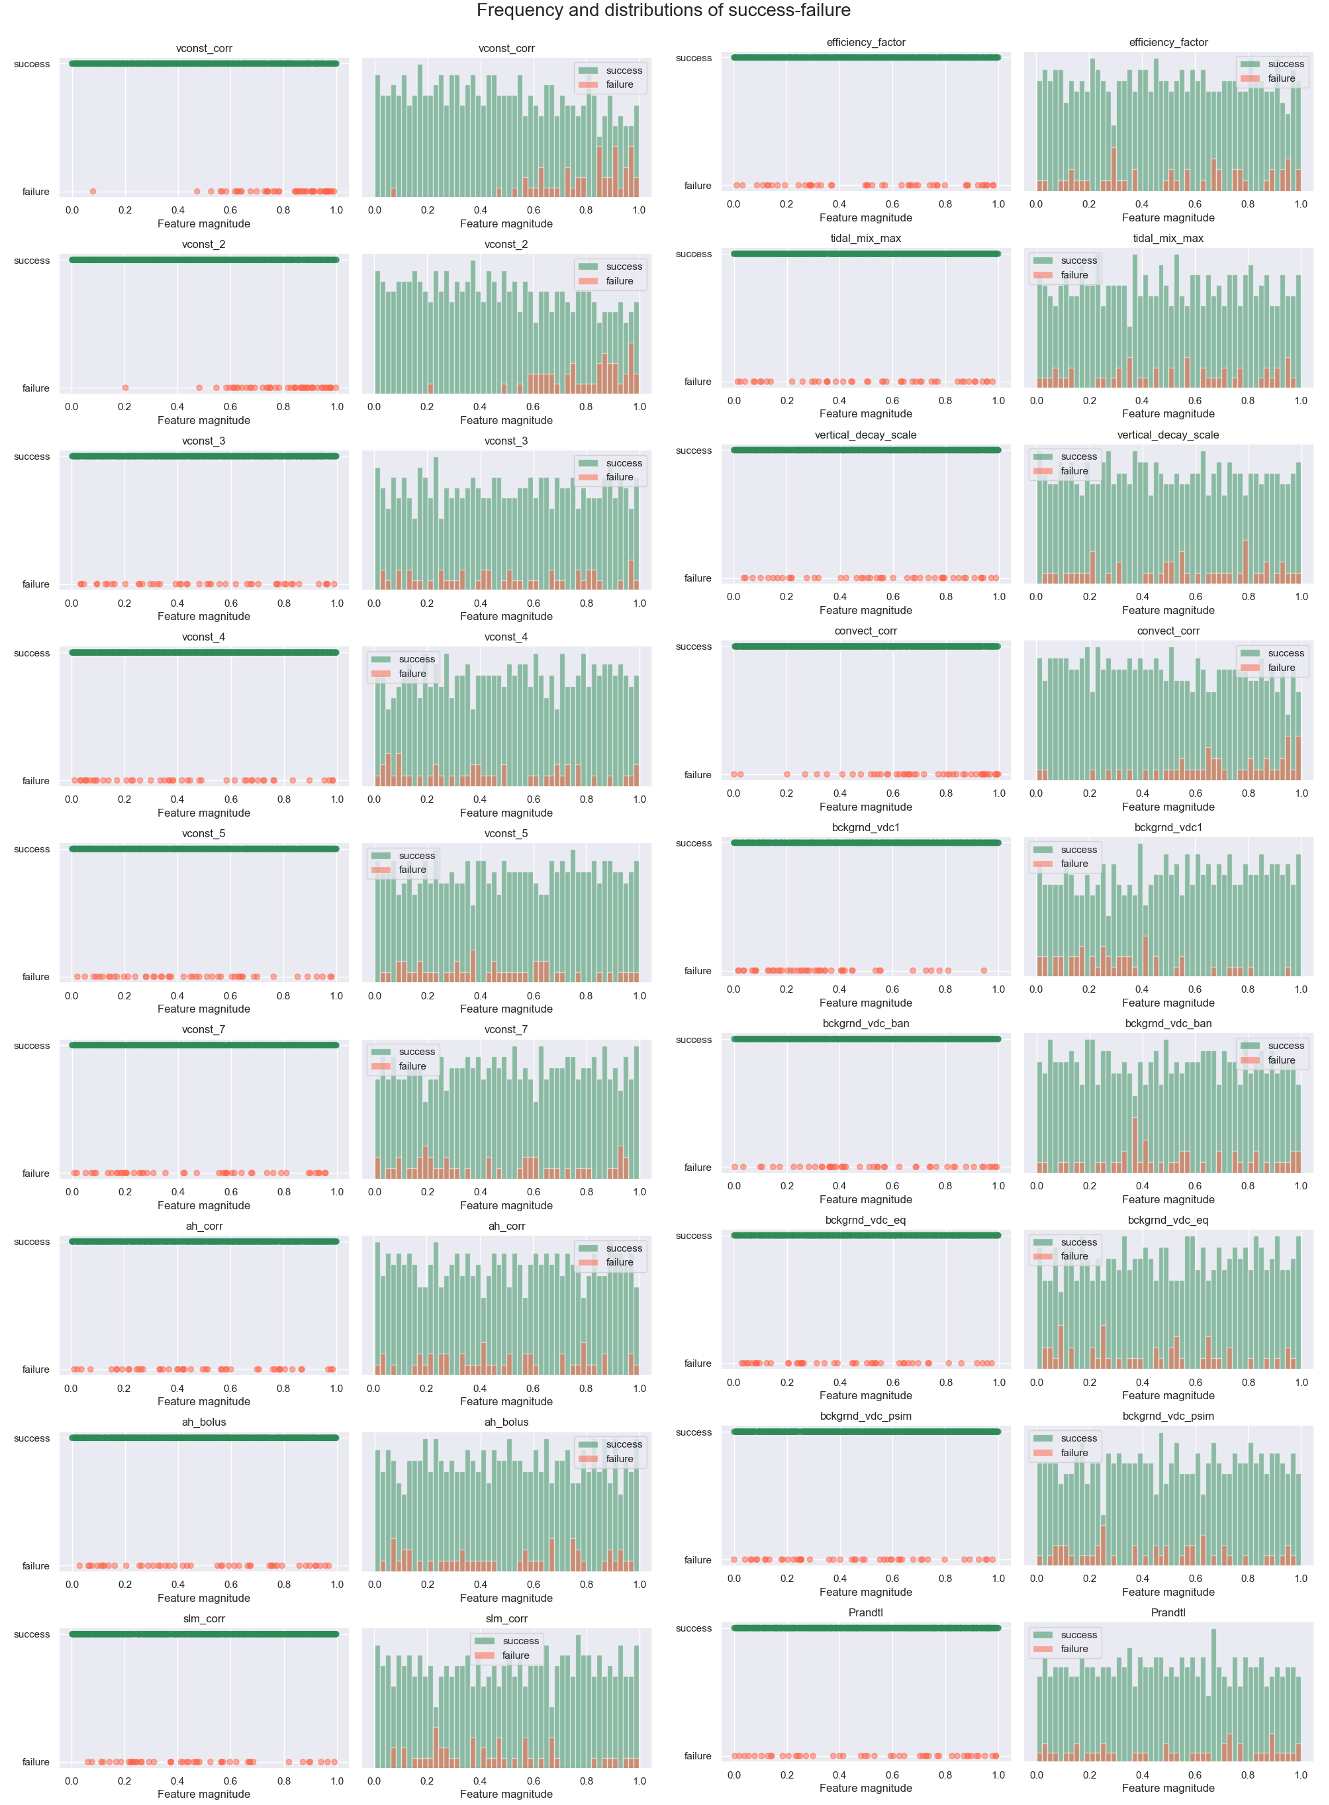
\includegraphics[scale=1.5]{dataset/distributions_tot.png}
    \caption{Total plot of the outcomes frequency and distribution for all 18 parameters.}
    \label{data:tot}
\end{figure}

\begin{figure}[h]
    \centering 
    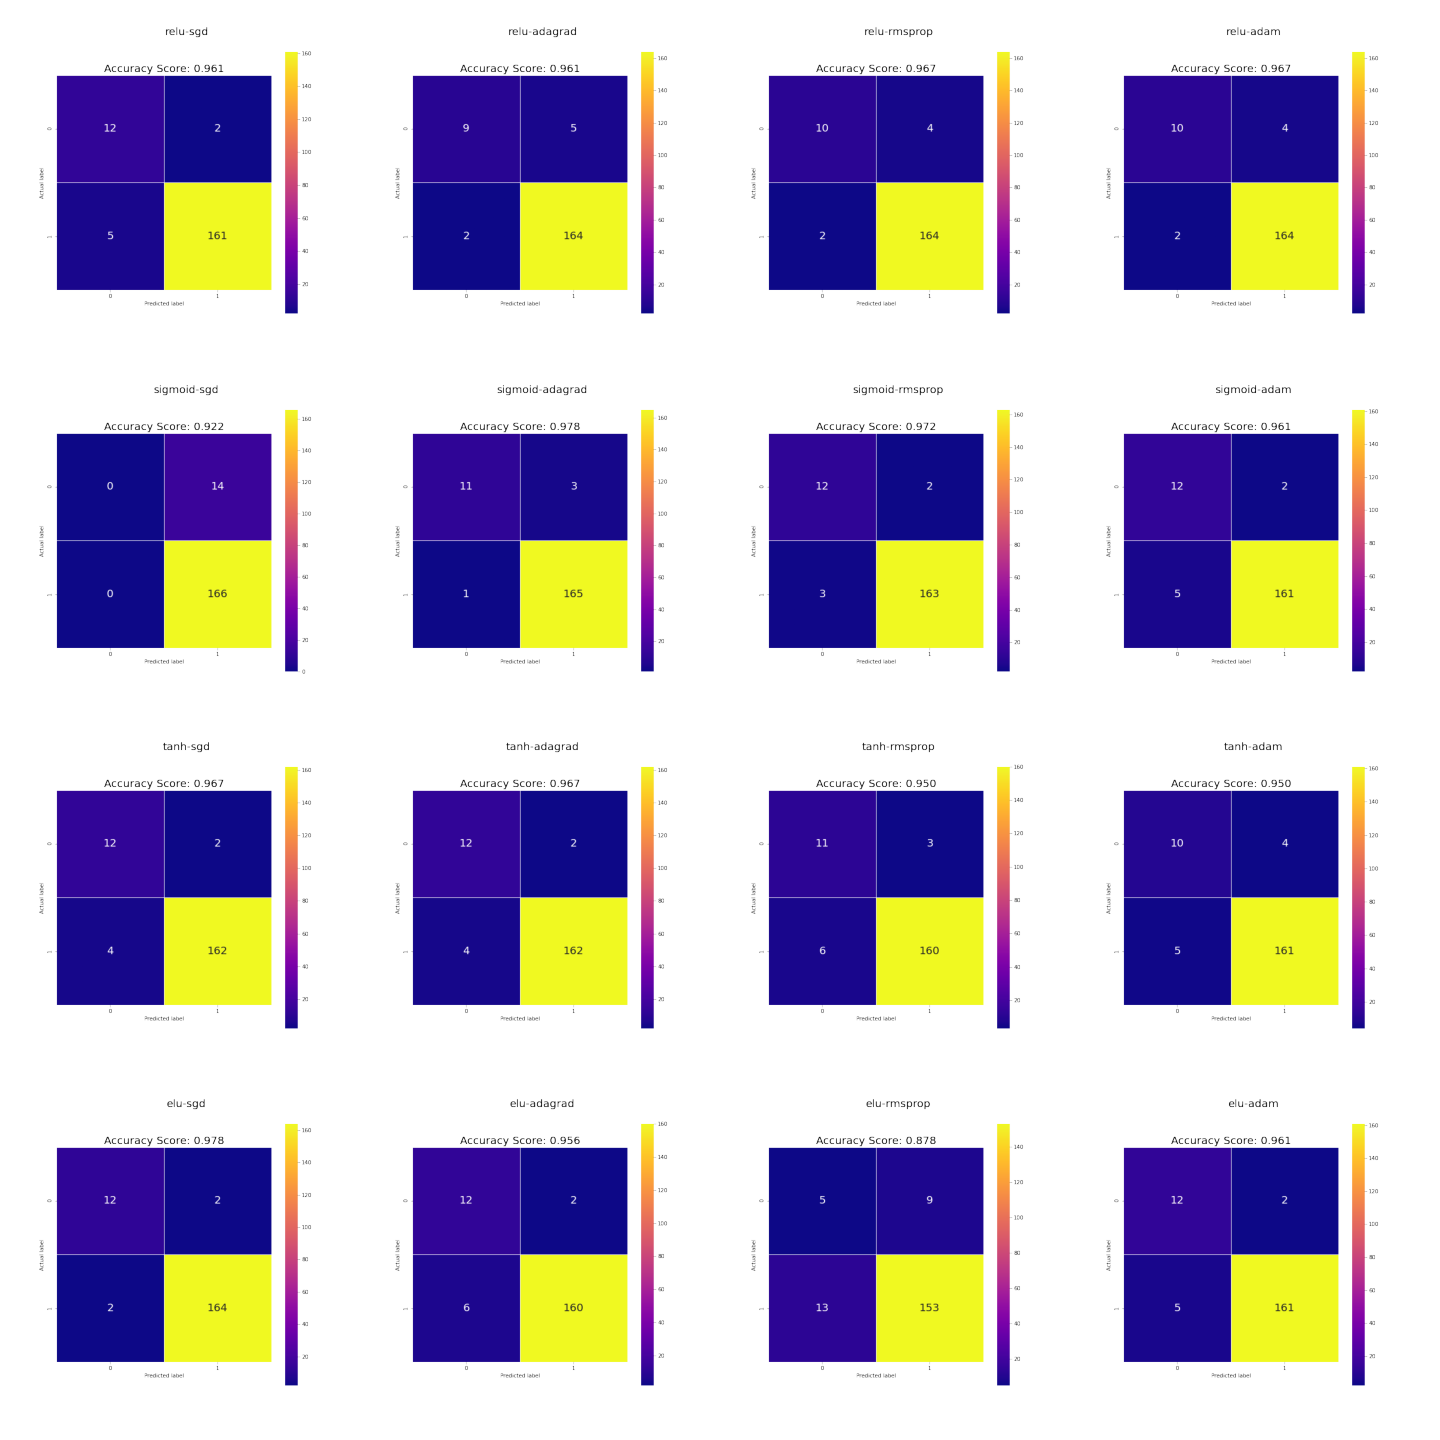
\includegraphics[scale=0.37]{results/confusionmatrix_nn_overall.png}
    \caption{Collection of all the 16 confusion matrix for the combination of the 4 activation functions (\textit{'relu', 'sigmoid','tanh','elu'}) and the 4 optimizers \textit{'sgd', 'adagrad','rmsprop','adam'}).}
    \label{res:nn_tot}
\end{figure}

\clearpage

\section*{References}\label{sec:references}
\bibliographystyle{unsrt}
\bibliography{bibliography.bib}


\end{document}

% ===========================================
https://neptune.ai/blog/how-to-compare-machine-learning-models-and-algorithms